\documentclass[11pt]{article}

\usepackage[utf8]{inputenc}
\usepackage[T1]{fontenc}
\usepackage[spanish,es-tabla]{babel}
\usepackage{lmodern}
\usepackage{microtype}
\usepackage{geometry}
\usepackage{graphicx}
\usepackage{float}
\usepackage{subcaption}
\usepackage{amsmath}
\usepackage{amssymb}
\usepackage{booktabs}
\usepackage{array}
\usepackage{adjustbox}
\usepackage{xcolor}
\usepackage{hyperref}
\usepackage{fancyhdr}
\usepackage{cite}

\geometry{bottom=3cm, top=3cm, left=3cm, right=3cm}
\setlength{\parskip}{0.55em}
\setlength{\parindent}{0pt}
\setlength{\headheight}{15pt}
\renewcommand{\arraystretch}{1.25}
\graphicspath{{./}{../figs/}}

\definecolor{myblue}{RGB}{0,0,128}
\definecolor{myred}{RGB}{128,0,0}

\hypersetup{
    colorlinks=true,
    linkcolor=myblue,
    citecolor=myred,
    filecolor=magenta,
    urlcolor=cyan
}

\pagestyle{fancy}
\fancyhf{}
\fancyhead[L]{\nouppercase{\leftmark}}
\fancyfoot[L]{\textit{Informe de Proyecto}}
\fancyfoot[C]{\thepage}
\fancyfoot[R]{\textit{Procesamiento Digital de Imágenes}}
\renewcommand{\headrulewidth}{0.4pt}
\renewcommand{\footrulewidth}{0.4pt}

\newcommand{\rankone}{\textit{Rank-1 Accuracy}}

\begin{document}

\hypersetup{pageanchor=false}
\begin{titlepage}
\centering
{\includegraphics[width=0.78\textwidth]{\detokenize{Portada/logo die (1) (1) (3) (1) (2) (2).png}}}
\vspace{1cm}

{\scshape\Large EL7007-1 Introducción al Procesamiento Digital de Imágenes \par}
\vspace{2.5cm}

{\scshape\Huge Informe de Proyecto\par}
\vspace{0.5cm}
{\scshape\Large Reconocimiento facial en imágenes de dron usando DroneFace y ArcFace\par}
\vspace{3.5cm}

\begin{flushright}
{\large Autores: Martín Aburto y Fernando Quintero\par}
\vspace{0.5cm}
{\large Profesor: Claudio Pérez Flores\par}
\vspace{0.5cm}
{\large Auxiliar: Christian Díaz Guerra\par}
\vspace{0.5cm}
{\large Ayudante: Renato Cariaga Cárcamo\par}
\vspace{0.5cm}
{\large Ayudante de Laboratorio: Juan Pablo Pérez Caballero\par}
\vspace{0.5cm}
{\large \today \par}
\vspace{0.5cm}
{\large Repositorio: \href{https://github.com/MartinInvi/Proyecto-EL7007-Reconocimiento-de-Rostros-desde-drones}{MartinInvi/Proyecto-EL7007-Reconocimiento-de-Rostros-desde-drones}\par}
\end{flushright}
\end{titlepage}

\clearpage
\hypersetup{pageanchor=true}
\pagenumbering{arabic}
\setcounter{page}{1}
\tableofcontents
\newpage

\section{Introducción}
\label{sec:introduccion}

El reconocimiento facial en imágenes capturadas desde drones es un problema más exigente que el reconocimiento en fotografías frontales controladas. La distancia a la cámara, la baja resolución efectiva del rostro, la borrosidad, la compresión y la variación de escala afectan tanto la detección facial como la extracción de descriptores. Por esta razón, un sistema evaluado únicamente con rostros ya recortados puede entregar una estimación optimista de desempeño.

Este proyecto construye un \textit{baseline} reproducible sobre DroneFace \cite{hsu2017droneface}. Se utiliza el paquete preentrenado \texttt{buffalo\_l} de InsightFace \cite{insightface2026,insightface_model_zoo}, que integra un submodelo de detección facial y un submodelo de reconocimiento basado en embeddings tipo ArcFace \cite{deng2019arcface}. No se entrena una red desde cero y tampoco se implementa control de dron. El objetivo es medir, con cuidado metodológico, qué parte del problema corresponde al reconocimiento facial y qué parte corresponde al paso previo de detectar y aislar rostros en imágenes completas.

Aunque inicialmente se consideró incluir SCface, ese dataset no se encuentra disponible localmente en esta etapa del proyecto. Por lo tanto, el alcance final del informe se concentra en DroneFace y en el problema de reconocimiento facial bajo captura aérea.

El trabajo se organiza en tres experimentos:

\begin{itemize}
    \item \textbf{Experimento A:} evaluación \textit{closed-set} sobre recortes de \texttt{photos\_all\_faces}.
    \item \textbf{Experimento B:} evaluación sobre imágenes completas de dron de \texttt{photos\_all}, reportada como recuperación de identidades esperadas a nivel de imagen completa.
    \item \textbf{Experimento C:} evaluación controlada con degradación sintética sobre imágenes con identidad conocida, para medir reconocimiento bajo ruido visual usando \rankone.
\end{itemize}

Las tres experiencias no usan exactamente las mismas métricas porque no responden la misma pregunta experimental. El Experimento A mide reconocimiento cuando el rostro ya viene recortado y la identidad real es conocida. El Experimento B mide el flujo completo sobre imágenes de dron, pero solo con etiquetas débiles a nivel de imagen; por eso no permite calcular TP, FP, FN ni F1 por rostro. El Experimento C se agrega como control: degrada imágenes con identidad conocida para medir de forma verificable la robustez del reconocimiento ante blur, compresión y baja resolución.

\section{Marco teórico}
\label{sec:marco}

\subsection{Reconocimiento facial basado en embeddings}

Los métodos modernos de reconocimiento facial suelen representar cada rostro mediante un vector numérico o \textit{embedding}. La comparación entre rostros se realiza en ese espacio: dos imágenes de la misma persona deberían quedar cerca, mientras que identidades distintas deberían quedar separadas. Este enfoque es común en modelos como FaceNet \cite{schroff2015facenet} y ArcFace \cite{deng2019arcface}.

En este proyecto se usa identificación \textit{closed-set}. Esto significa que cada rostro evaluado pertenece a una identidad que ya está presente en la galería. Dado un embedding de prueba $\mathbf{x}$ y una galería de embeddings $\{\mathbf{g}_i\}$, se predice la identidad con mayor similitud coseno:

\begin{equation}
    \operatorname{sim}(\mathbf{x}, \mathbf{g}_i)
    =
    \frac{\mathbf{x}^{T}\mathbf{g}_i}{\|\mathbf{x}\|_2\|\mathbf{g}_i\|_2}.
\end{equation}

La predicción final corresponde a:

\begin{equation}
    \hat{y} = \arg\max_i \operatorname{sim}(\mathbf{x}, \mathbf{g}_i).
\end{equation}

No se utiliza umbral de ``desconocido''. Por lo tanto, cuando existe una detección válida, el sistema siempre asigna la imagen a la identidad más parecida dentro de la galería.

\subsection{ArcFace, detección facial e InsightFace}

ArcFace introduce una pérdida con margen angular aditivo para obtener embeddings más discriminativos \cite{deng2019arcface}. En vez de optimizar únicamente la clasificación de identidades, fuerza una separación angular más clara entre clases. En este proyecto, ArcFace no se implementa manualmente: se usa mediante InsightFace, una biblioteca de análisis facial que entrega un flujo completo de detección, alineamiento y extracción de embeddings \cite{insightface2026}.

Es importante distinguir entre el paquete usado y las redes internas. Se usa el mismo paquete \texttt{buffalo\_l} durante todo el proyecto, pero eso no significa que la misma red neuronal haga detección y reconocimiento. Según el \textit{model zoo} de InsightFace, \texttt{buffalo\_l} combina un detector facial RetinaFace-10GF con un reconocedor ResNet50 entrenado sobre WebFace600K \cite{insightface_model_zoo}. En la ejecución local, InsightFace carga archivos ONNX separados: \texttt{det\_10g.onnx} para detección y \texttt{w600k\_r50.onnx} para reconocimiento.

La etapa de detección entrega cajas delimitadoras, puntajes de confianza y puntos de alineamiento. RetinaFace es un detector de una etapa que combina localización facial y puntos faciales, lo que permite alimentar al reconocedor con rostros alineados \cite{deng2020retinaface}. Luego, el reconocedor recibe el rostro alineado, genera un embedding y este vector se compara con la galería usando similitud coseno.

\subsection{Particularidades de DroneFace}

DroneFace contiene imágenes capturadas en condiciones relacionadas con dron, incluyendo variaciones de distancia y altura \cite{hsu2017droneface}. En este proyecto se usan tres carpetas principales:

\begin{itemize}
    \item \texttt{portraits}: retratos limpios usados como galería.
    \item \texttt{photos\_all\_faces}: rostros ya recortados usados como \textit{probes} del Experimento A.
    \item \texttt{photos\_all}: imágenes completas del dron usadas en el Experimento B.
\end{itemize}

La composición local del dataset se resume en la Tabla~\ref{tab:dataset_local}. Esta tabla es importante porque la copia usada no contiene retratos en \texttt{portraits} para los 11 sujetos de DroneFace. En consecuencia, las métricas de reconocimiento se calculan solo sobre identidades con galería disponible.

\begin{table}[H]
\centering
\caption{Composición del dataset DroneFace disponible localmente.}
\label{tab:dataset_local}
\begin{adjustbox}{max width=\textwidth}
\begin{tabular}{lcl}
\toprule
Carpeta & Imágenes & Uso en este informe \\
\midrule
\texttt{portraits} & 7 & Galería de identidades conocidas \\
\texttt{photos\_all\_faces} & 1364 & Probes recortados; 868 evaluados y 496 excluidos por no tener galería \\
\texttt{photos\_all} & 620 & Imágenes completas para el Experimento B \\
\texttt{trio\_cam} & 33 & No usado; requiere definir un protocolo adicional de galería multi-vista/cámara \\
\texttt{trio\_gp} & 33 & No usado; requiere definir un protocolo adicional de galería multi-vista/cámara \\
\bottomrule
\end{tabular}
\end{adjustbox}
\end{table}

Las carpetas \texttt{trio\_cam} y \texttt{trio\_gp} contienen vistas frontales y laterales adicionales. Se dejan fuera de la evaluación principal para no mezclar protocolos de galería: el baseline reportado usa únicamente los retratos disponibles en \texttt{portraits}.

\section{Metodología}
\label{sec:metodologia}

\subsection{Configuración experimental del modelo}

La Tabla~\ref{tab:config_modelo} aclara la configuración usada. El flujo usa InsightFace \texttt{FaceAnalysis} con el paquete \texttt{buffalo\_l}. La detección y el reconocimiento pertenecen al mismo paquete, pero son submodelos distintos: el detector encuentra rostros y produce cajas; el reconocedor convierte cada rostro alineado en un embedding. El parámetro ajustado experimentalmente fue \texttt{det\_size}, que se entrega a \texttt{app.prepare(..., det\_size=...)} y controla el tamaño de entrada usado por el detector. Este parámetro no reentrena el modelo ni cambia directamente la dimensión del embedding de reconocimiento.

\begin{table}[H]
\centering
\caption{Configuración del modelo y selección de \texttt{det\_size}.}
\label{tab:config_modelo}
\begin{adjustbox}{max width=\textwidth}
\begin{tabular}{llll}
\toprule
Componente o protocolo & Configuración usada & Rol & Motivo de uso \\
\midrule
Detector facial & \texttt{buffalo\_l} / \texttt{det\_10g.onnx} & Generar cajas y puntajes & RetinaFace-10GF incluido en InsightFace \\
Reconocedor facial & \texttt{buffalo\_l} / \texttt{w600k\_r50.onnx} & Generar embeddings & Backbone ResNet50@WebFace600K del paquete \texttt{buffalo\_l} \\
Experimentos A y C & \texttt{det\_size=(320, 320)} & Rostros recortados & Mejor configuración del barrido en recortes \\
Experimento B & \texttt{det\_size=(1280, 1280)} & Imágenes completas & Mejor recuperación en rostros pequeños de imágenes de dron \\
\bottomrule
\end{tabular}
\end{adjustbox}
\end{table}

Como se verá en las Tablas~\ref{tab:det_size_a} y~\ref{tab:det_size_b}, la configuración final no se eligió arbitrariamente. En recortes faciales, \texttt{det\_size=320} obtiene la mayor \texttt{accuracy\_global}; en imágenes completas, \texttt{det\_size=1280} obtiene la mayor tasa de detección por imagen y la mayor recuperación de identidades esperadas.

\subsection{Reproducibilidad experimental}

La Tabla~\ref{tab:reproducibilidad} resume los elementos necesarios para reproducir el protocolo. El código fuerza ejecución en CPU mediante \texttt{allow\_cuda=False}, por lo que InsightFace se ejecuta con \texttt{CPUExecutionProvider}. El archivo \texttt{requirements.txt} lista dependencias, pero no fija versiones exactas; por esta razón, no se reportan números de versión que no estén controlados por el repositorio.

\begin{table}[H]
\centering
\caption{Configuración de reproducibilidad del experimento.}
\label{tab:reproducibilidad}
\begin{adjustbox}{max width=\textwidth}
\begin{tabular}{ll}
\toprule
Elemento & Valor usado \\
\midrule
Modelo de InsightFace & \texttt{buffalo\_l} \\
Detector & \texttt{det\_10g.onnx} \\
Reconocedor & \texttt{w600k\_r50.onnx} \\
Proveedor de ejecución & \texttt{CPUExecutionProvider} \\
Repositorio del proyecto & \href{https://github.com/MartinInvi/Proyecto-EL7007-Reconocimiento-de-Rostros-desde-drones}{MartinInvi/Proyecto-EL7007-Reconocimiento-de-Rostros-desde-drones} \\
Dependencias principales & \texttt{numpy}, \texttt{pandas}, \texttt{matplotlib}, \texttt{opencv-python}, \texttt{scikit-learn}, \texttt{tqdm}, \texttt{jupyter}, \texttt{insightface}, \texttt{onnxruntime} \\
\bottomrule
\end{tabular}
\end{adjustbox}
\end{table}

\subsection{Construcción de galería}

La galería se construye con las imágenes de \texttt{portraits}. Para cada sujeto disponible se detecta el rostro, se extrae el embedding y se almacena el vector normalizado. En la copia local usada solo existen retratos para 7 sujetos: \texttt{a}, \texttt{d}, \texttt{e}, \texttt{g}, \texttt{i}, \texttt{j} y \texttt{k}. Los sujetos \texttt{b}, \texttt{c}, \texttt{f} y \texttt{h} aparecen en \texttt{photos\_all} y \texttt{photos\_all\_faces}, pero no tienen retrato en \texttt{portraits}; por lo tanto, no existe embedding de galería contra el cual compararlos.

\begin{table}[H]
\centering
\caption{Disponibilidad de galería por sujeto en la copia local de DroneFace.}
\label{tab:sujetos_galeria}
\begin{tabular}{cccc}
\toprule
Sujeto & Tiene \texttt{portrait} local & Embedding válido & Uso en galería \\
\midrule
\texttt{a} & Sí & Sí & Sí \\
\texttt{b} & No & No aplica & No \\
\texttt{c} & No & No aplica & No \\
\texttt{d} & Sí & Sí & Sí \\
\texttt{e} & Sí & Sí & Sí \\
\texttt{f} & No & No aplica & No \\
\texttt{g} & Sí & Sí & Sí \\
\texttt{h} & No & No aplica & No \\
\texttt{i} & Sí & Sí & Sí \\
\texttt{j} & Sí & Sí & Sí \\
\texttt{k} & Sí & Sí & Sí \\
\bottomrule
\end{tabular}
\end{table}

La Tabla~\ref{tab:sujetos_galeria} muestra que la restricción viene de la disponibilidad local de retratos, no de una falla del modelo. El archivo \texttt{gallery\_failures\_droneface.csv} no reporta fallas de construcción de galería; los sujetos excluidos simplemente no tienen imagen de referencia en \texttt{portraits}. Por esta razón, las métricas de reconocimiento de A, B y C se definen solo sobre identidades con galería.

\subsection{Experimento A: rostros recortados}

El Experimento A busca aislar el módulo de reconocimiento cuando el problema de localización del rostro ya está casi resuelto por el propio dataset. Evalúa el sistema sobre \texttt{photos\_all\_faces}, donde cada imagen contiene un rostro recortado y una identidad conocida. Solo se evalúan sujetos presentes en la galería. Por lo tanto, se evalúan 868 probes correspondientes a \texttt{a}, \texttt{d}, \texttt{e}, \texttt{g}, \texttt{i}, \texttt{j} y \texttt{k}; los 496 probes de \texttt{b}, \texttt{c}, \texttt{f} y \texttt{h} se excluyen porque no existe referencia en \texttt{portraits}. Para cada probe:

\begin{enumerate}
    \item se detecta el rostro;
    \item se extrae su embedding;
    \item se compara contra todos los embeddings de galería usando similitud coseno;
    \item se asigna la identidad con mayor similitud.
\end{enumerate}

Las métricas usadas son:

\begin{align}
    \text{detection\_rate} &= \frac{\text{rostros detectados}}{\text{total de probes}}, \\
    \text{accuracy\_conditional} &= \frac{\text{aciertos}}{\text{rostros detectados}}, \\
    \text{accuracy\_global} &= \frac{\text{aciertos}}{\text{total de probes}}.
\end{align}

La métrica principal es \texttt{accuracy\_global}, ya que penaliza tanto errores de reconocimiento como fallas de detección.

\subsection{Experimento B: imágenes completas con supervisión débil}

El Experimento B busca aproximar el caso real de uso: partir desde una imagen completa de dron, detectar rostros pequeños y recuperar identidades presentes. Usa \texttt{photos\_all}. En estas imágenes la etiqueta puede ser compuesta, por ejemplo \texttt{ab}, \texttt{cd}, \texttt{ef}, \texttt{gh} o \texttt{ijk}. Esto indica qué identidades aparecen en la imagen, pero no entrega la identidad asociada a cada bounding box.

Por esa razón, en este experimento no se reportan TP, FP, FN, precisión ni F1 por rostro. Esas métricas requerirían saber manualmente qué persona corresponde a cada caja detectada. En su lugar, se reporta recuperación de identidades esperadas a nivel de imagen completa.

Para cada imagen se calcula:

\begin{equation}
    \text{expected\_identity\_recall}
    =
    \frac{|\mathcal{E} \cap \mathcal{P}|}{|\mathcal{E}|},
\end{equation}

donde $\mathcal{E}$ es el conjunto de identidades esperadas con galería y $\mathcal{P}$ es el conjunto de identidades predichas por el sistema. Las identidades esperadas sin galería se registran aparte y no entran al denominador de recuperación. Además, $\mathcal{P}$ se calcula como un conjunto de identidades únicas por imagen: si el sistema predice la misma identidad en varias detecciones de una imagen, esa identidad se cuenta una sola vez para \texttt{expected\_identity\_recall} y Jaccard. Se reporta la similitud de Jaccard \cite{jaccard1901}, una medida estándar de solapamiento entre conjuntos:

\begin{equation}
    J(\mathcal{E}, \mathcal{P}) =
    \frac{|\mathcal{E} \cap \mathcal{P}|}{|\mathcal{E} \cup \mathcal{P}|}.
\end{equation}

Las identidades predichas que no pertenecen al conjunto esperado se informan como \textit{identidades inesperadas}. No se llaman falsos positivos, porque no existe verificación manual por rostro.

\subsection{Experimento C: degradación sintética controlada}

El Experimento C fue agregado para responder una pregunta distinta: qué tan robusto es el módulo de reconocimiento cuando la identidad real sí es conocida y se controla artificialmente el ruido visual. Se toman probes de \texttt{photos\_all\_faces} de sujetos con galería que el Experimento A reconoce correctamente y se generan versiones degradadas en memoria. Por diseño, este experimento mide sensibilidad relativa frente a degradación visual en casos inicialmente reconocibles; no estima el desempeño absoluto sobre todo DroneFace. Las degradaciones aplicadas son:

\begin{itemize}
    \item reducción de resolución y reescalado;
    \item desenfoque gaussiano;
    \item compresión JPEG;
    \item traslación leve.
\end{itemize}

No se aplica rotación en esta versión para aislar degradaciones más directamente asociadas a resolución, compresión y blur. La métrica principal es:

\begin{equation}
    \text{rank1\_accuracy\_global}
    =
    \frac{\text{predicciones correctas}}{\text{total de probes sintéticos}}.
\end{equation}

También se reportan \texttt{detection\_rate} y \texttt{rank1\_accuracy\_conditional}. Este experimento no reemplaza el etiquetado manual de B, pero entrega una medición honesta del reconocimiento bajo ruido visual controlado.

\section{Resultados}
\label{sec:resultados}

\subsection{Resumen global}

La Tabla~\ref{tab:resumen_exp} resume la métrica principal de cada experimento. La diferencia entre las métricas no es un cambio cosmético: responde a la unidad evaluada y al tipo de anotación disponible. En A la unidad es un rostro recortado con identidad conocida; en B la unidad es una imagen completa con etiquetas débiles; en C la unidad es un probe sintético cuya identidad se conoce de forma controlada.

\begin{table}[H]
\centering
\caption{Resumen de métricas principales por experimento.}
\label{tab:resumen_exp}
\begin{adjustbox}{max width=\textwidth}
\begin{tabular}{llccc}
\toprule
Experimento & Unidad evaluada & Total & Métrica principal & Valor \\
\midrule
A & Rostro recortado & 868 probes & \texttt{accuracy\_global} & 90.78\% \\
B & Imagen completa & 620 imágenes & \texttt{expected\_identity\_recall\_global} & 78.80\% \\
C & Probe degradado & 210 por nivel & Rank-1 global, nivel \texttt{strong} & 74.29\% \\
\bottomrule
\end{tabular}
\end{adjustbox}
\end{table}

\subsection{Experimento A}

Como se muestra en la Tabla~\ref{tab:exp_a_global}, el Experimento A obtuvo una tasa de detección de 99.31\%, con 788 aciertos sobre 868 probes evaluados. La exactitud global fue 90.78\% y la exactitud condicional, calculada solo sobre rostros detectados, fue 91.42\%. La cercanía entre ambas métricas indica que, en recortes, el detector falla pocas veces; el error principal proviene de confusiones de reconocimiento en condiciones más difíciles.

\begin{table}[H]
\centering
\caption{Resultados globales del Experimento A.}
\label{tab:exp_a_global}
\begin{tabular}{lcc}
\toprule
Métrica & Valor absoluto & Proporción \\
\midrule
Probes evaluados & 868 & -- \\
Rostros detectados & 862 & 99.31\% \\
Predicciones correctas & 788 & 90.78\% del total \\
\texttt{accuracy\_conditional} & -- & 91.42\% \\
\texttt{accuracy\_global} & -- & 90.78\% \\
\bottomrule
\end{tabular}
\end{table}

La Figura~\ref{fig:det_acc_a} muestra visualmente esta separación entre detección y reconocimiento: la tasa de detección es más alta que la exactitud global, por lo que el cuello de botella de A no es tanto encontrar el rostro, sino reconocer correctamente algunas identidades cuando la imagen se degrada.

La Tabla~\ref{tab:exp_a_sujeto} desagrega el resultado por sujeto. El desempeño no es uniforme: \texttt{a} y \texttt{e} son los sujetos más estables, mientras que \texttt{g} y \texttt{k} concentran más errores de reconocimiento. Este análisis es útil porque el promedio global puede ocultar diferencias asociadas a la representatividad del retrato de galería o a la apariencia de cada sujeto bajo distintas condiciones de captura.

\begin{table}[H]
\centering
\caption{Resultados del Experimento A por sujeto con galería.}
\label{tab:exp_a_sujeto}
\begin{tabular}{ccccc}
\toprule
Sujeto & Probes & Detectados & Correctos & \texttt{accuracy\_global} \\
\midrule
\texttt{a} & 124 & 124 & 124 & 100.00\% \\
\texttt{d} & 124 & 124 & 110 & 88.71\% \\
\texttt{e} & 124 & 124 & 121 & 97.58\% \\
\texttt{g} & 124 & 124 & 103 & 83.06\% \\
\texttt{i} & 124 & 119 & 112 & 90.32\% \\
\texttt{j} & 124 & 124 & 113 & 91.13\% \\
\texttt{k} & 124 & 123 & 105 & 84.68\% \\
\bottomrule
\end{tabular}
\end{table}

\begin{figure}[H]
\centering
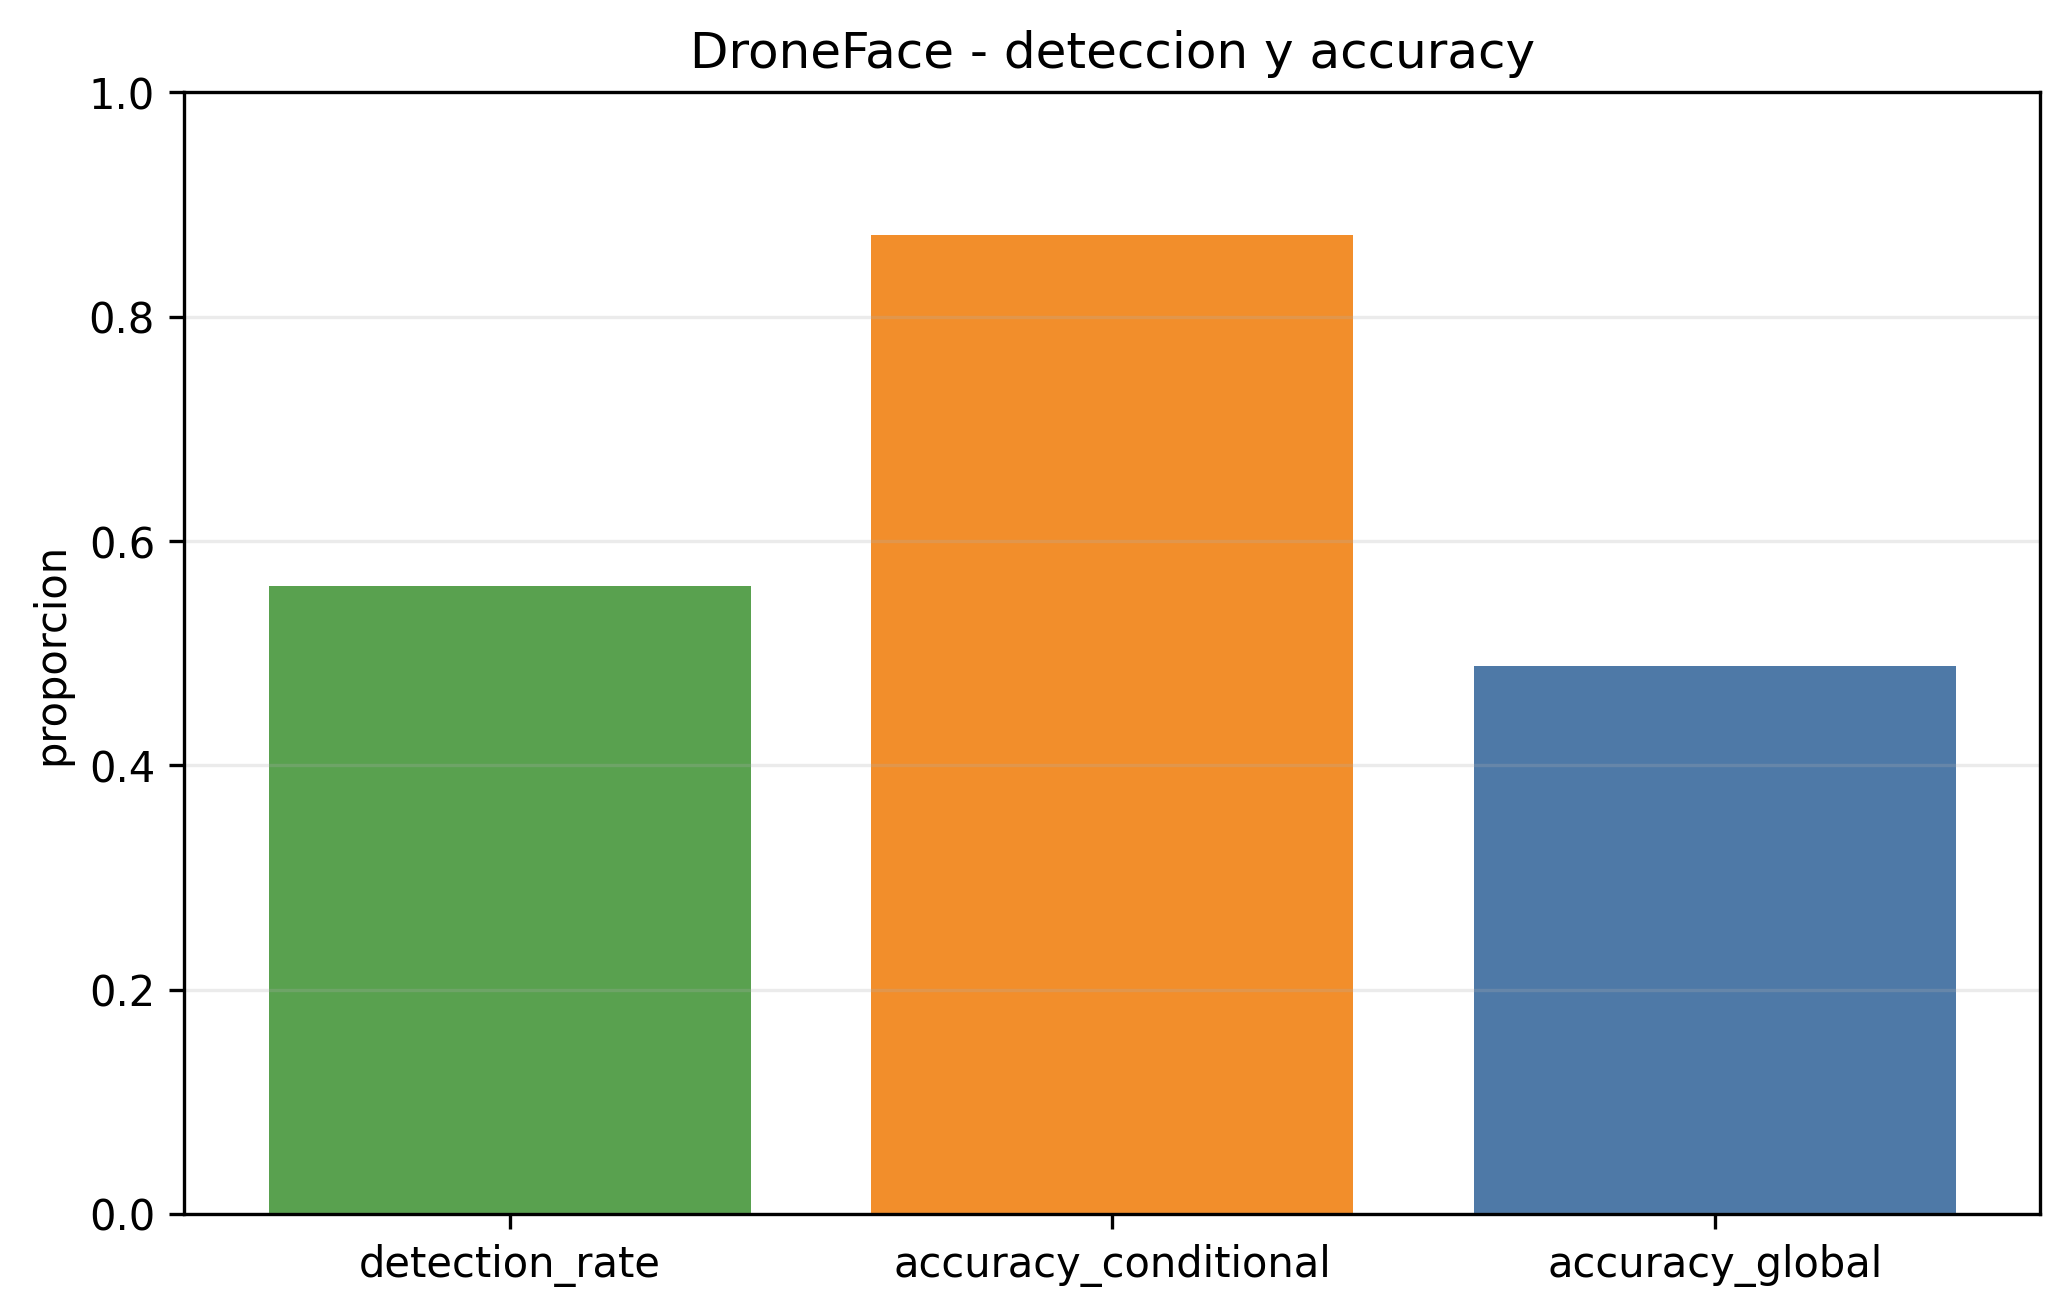
\includegraphics[width=0.88\textwidth]{metrics/droneface_detection_vs_accuracy.png}
\caption{Relación entre tasa de detección, exactitud condicional y exactitud global en el Experimento A.}
\label{fig:det_acc_a}
\end{figure}

La Figura~\ref{fig:exp_a_altura} muestra el desempeño por altura y la Figura~\ref{fig:exp_a_distancia} lo muestra por distancia. La exactitud disminuye especialmente al aumentar la distancia: la peor distancia agregada fue 17.0 m, con 60.71\% de \texttt{accuracy\_global}. Por altura, la peor condición agregada fue 5.0 m, con 86.64\%. Esto es consistente con la pérdida de resolución efectiva del rostro.

\begin{figure}[H]
\centering
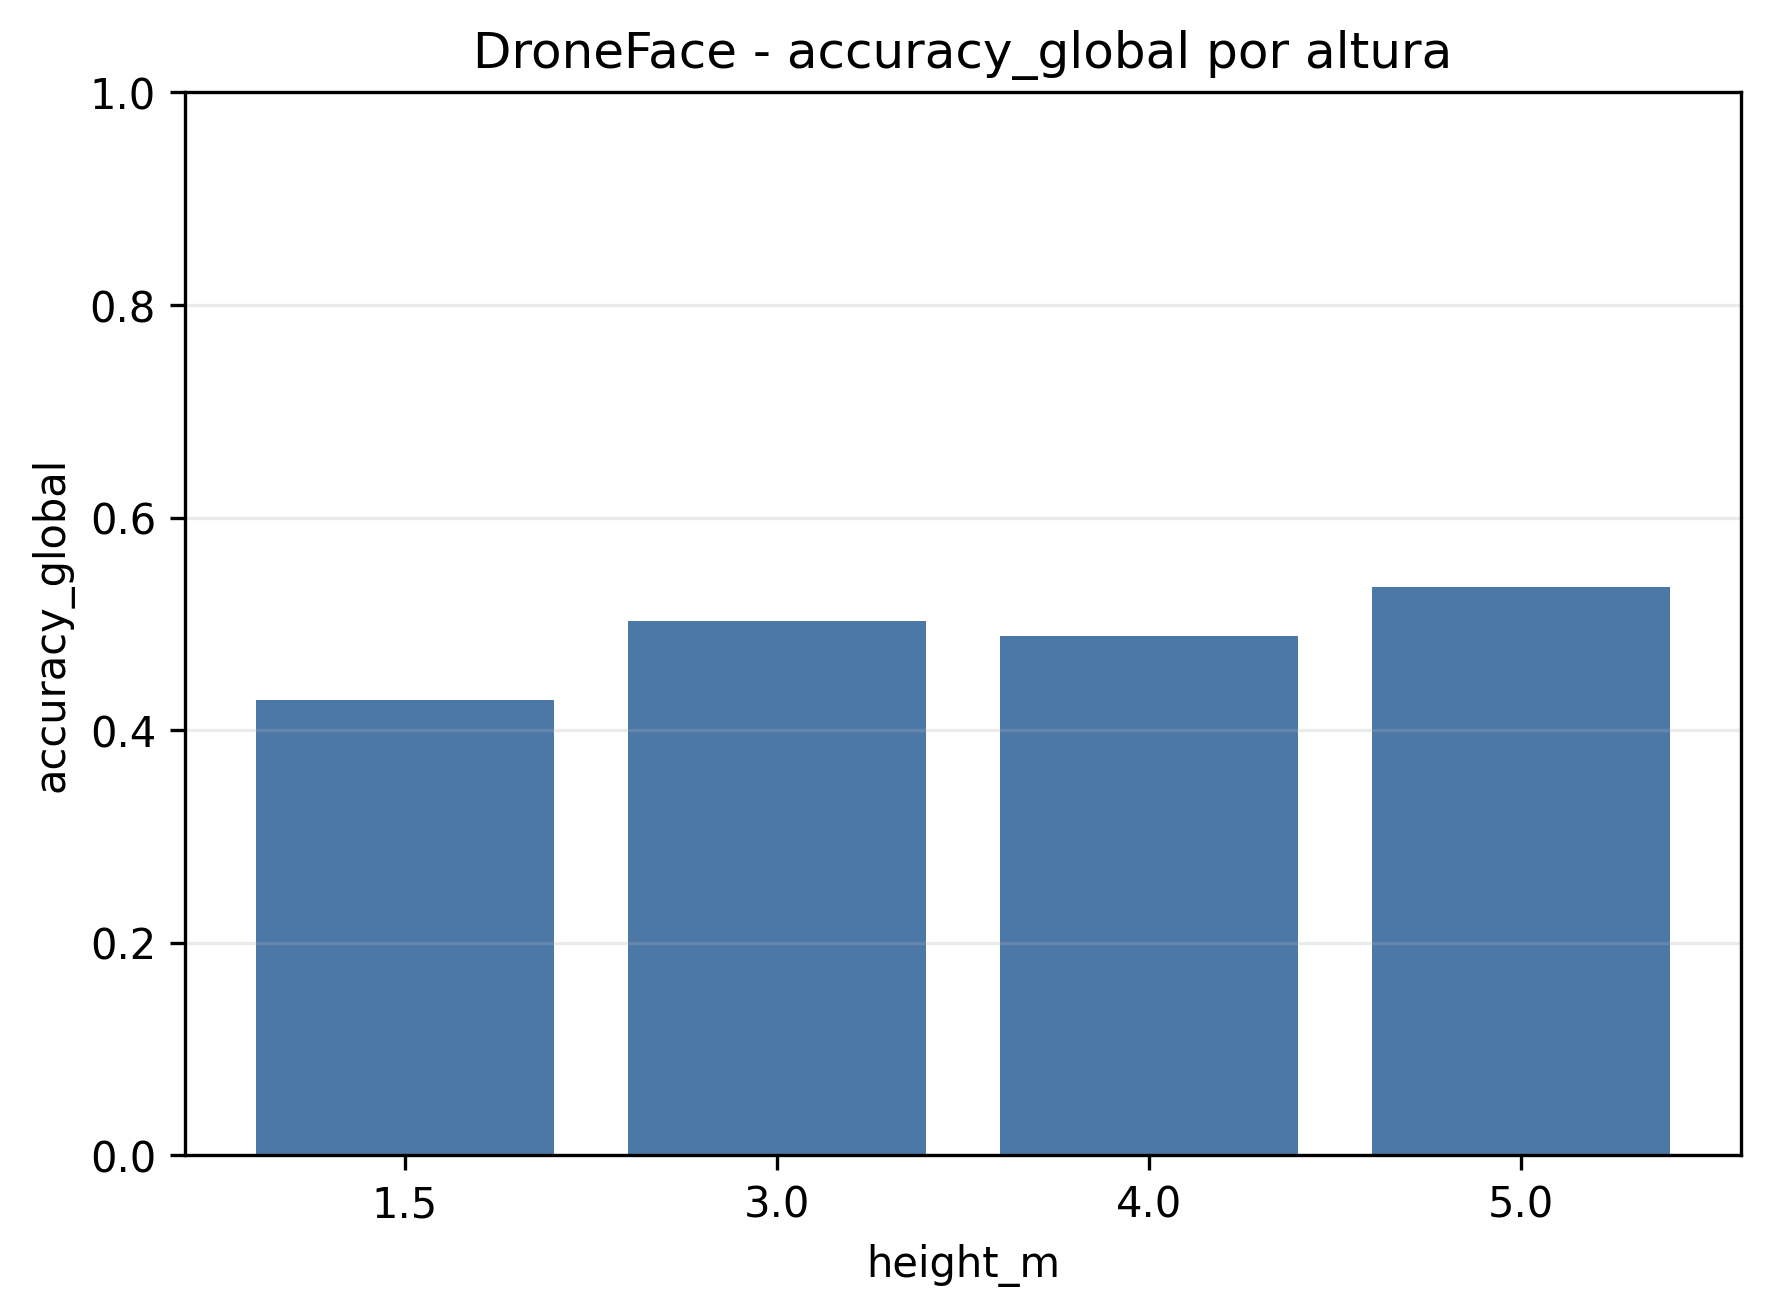
\includegraphics[width=0.95\textwidth]{metrics/droneface_accuracy_by_height.png}
\caption{Desempeño del Experimento A por altura de captura.}
\label{fig:exp_a_altura}
\end{figure}

\begin{figure}[H]
\centering
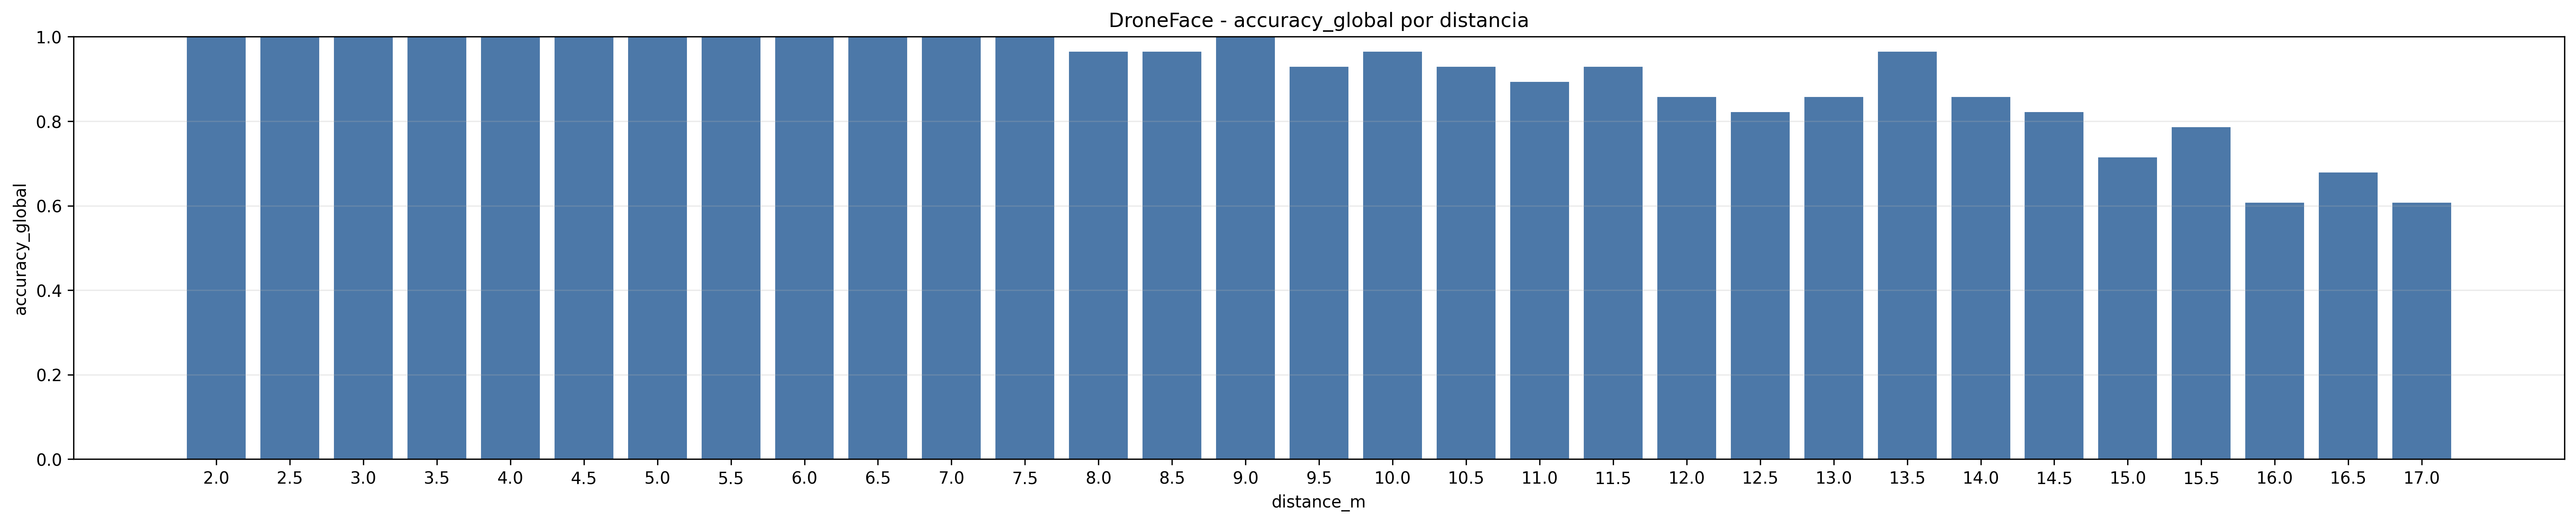
\includegraphics[width=0.95\textwidth]{metrics/droneface_accuracy_by_distance.png}
\caption{Desempeño del Experimento A por distancia de captura.}
\label{fig:exp_a_distancia}
\end{figure}

La Figura~\ref{fig:heatmap_a} combina altura y distancia. El mapa confirma que las condiciones de mayor distancia concentran las caídas más fuertes, incluso cuando la detección sigue funcionando en la mayoría de los recortes.

\begin{figure}[H]
\centering
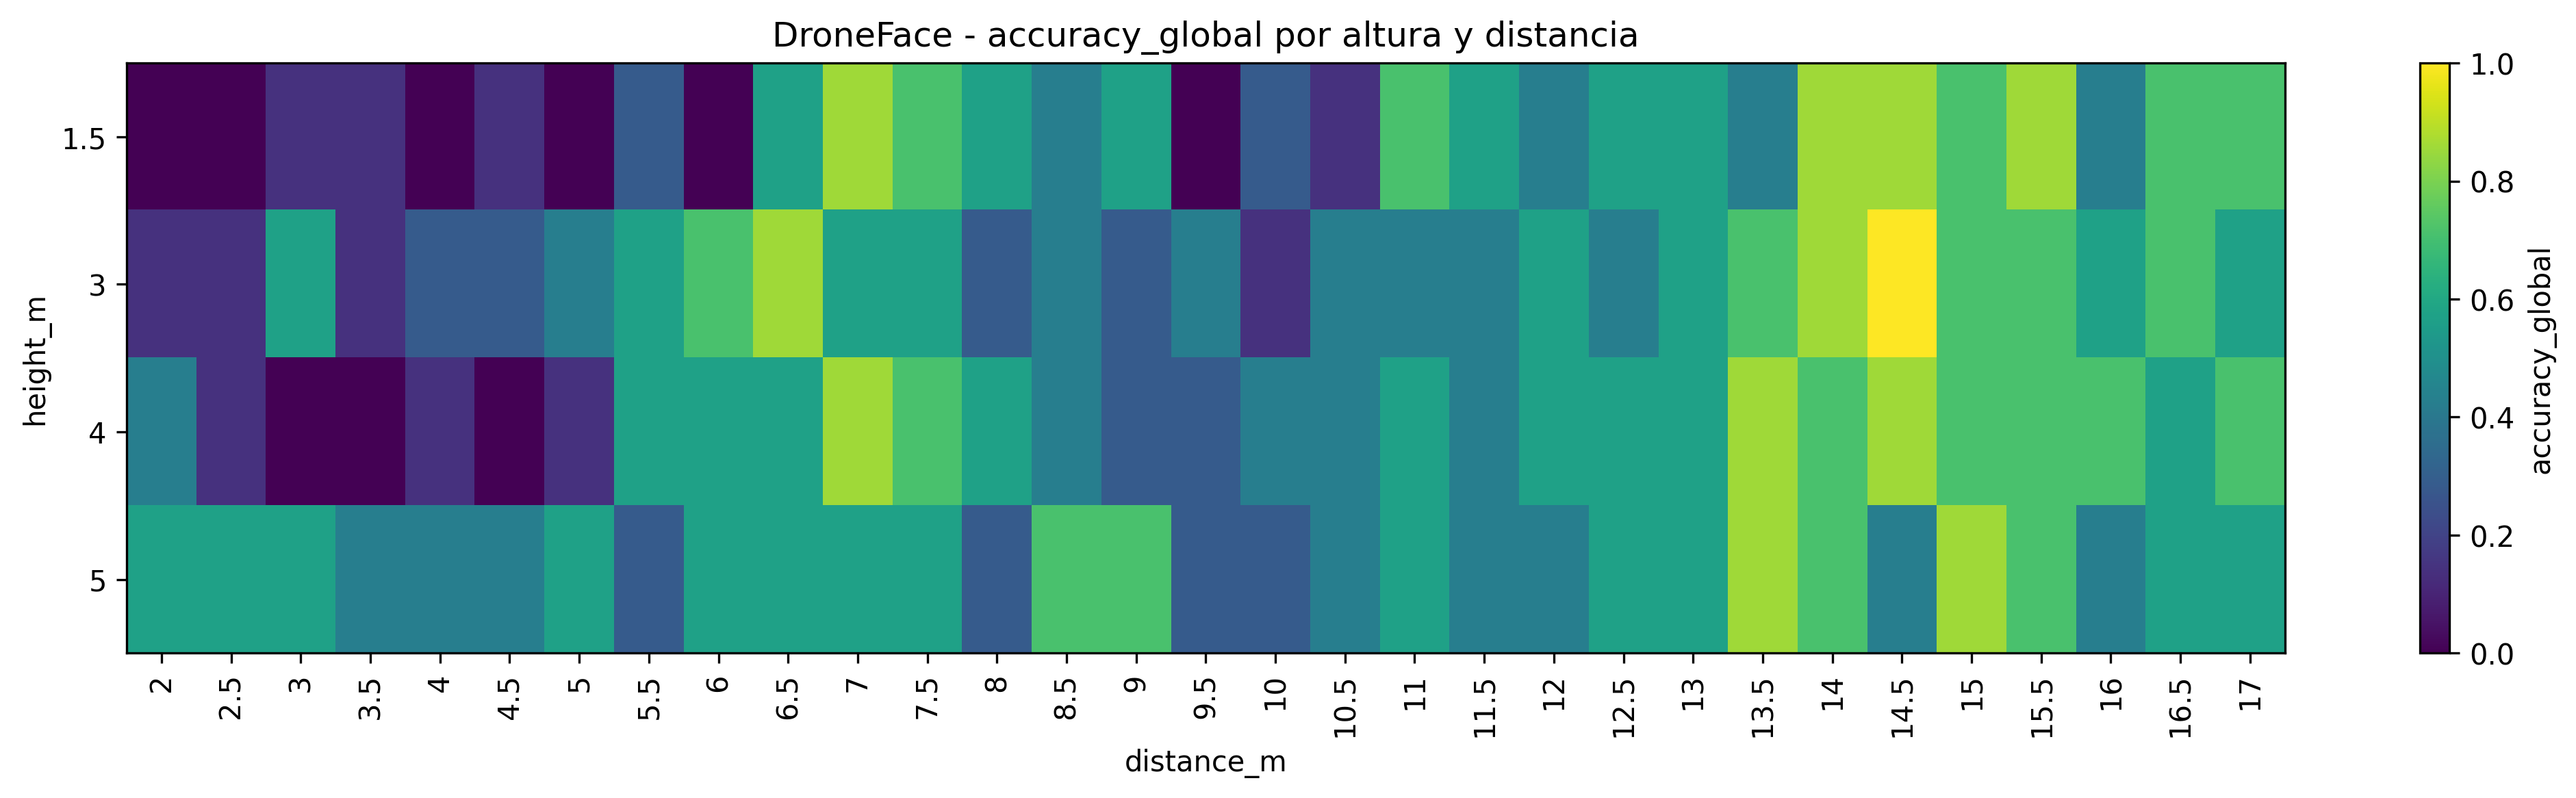
\includegraphics[width=\textwidth]{metrics/droneface_accuracy_height_distance.png}
\caption{Mapa de calor de \texttt{accuracy\_global} para el Experimento A por altura y distancia.}
\label{fig:heatmap_a}
\end{figure}

La Figura~\ref{fig:confusion_a} muestra la matriz de confusión del Experimento A. Las confusiones más frecuentes fueron \texttt{k}$\rightarrow$\texttt{e} con 17 casos, \texttt{g}$\rightarrow$\texttt{d} con 12 casos, \texttt{d}$\rightarrow$\texttt{j} con 12 casos y \texttt{j}$\rightarrow$\texttt{e} con 6 casos. Esto confirma que los errores no se distribuyen de manera completamente uniforme entre identidades.

\begin{figure}[H]
\centering
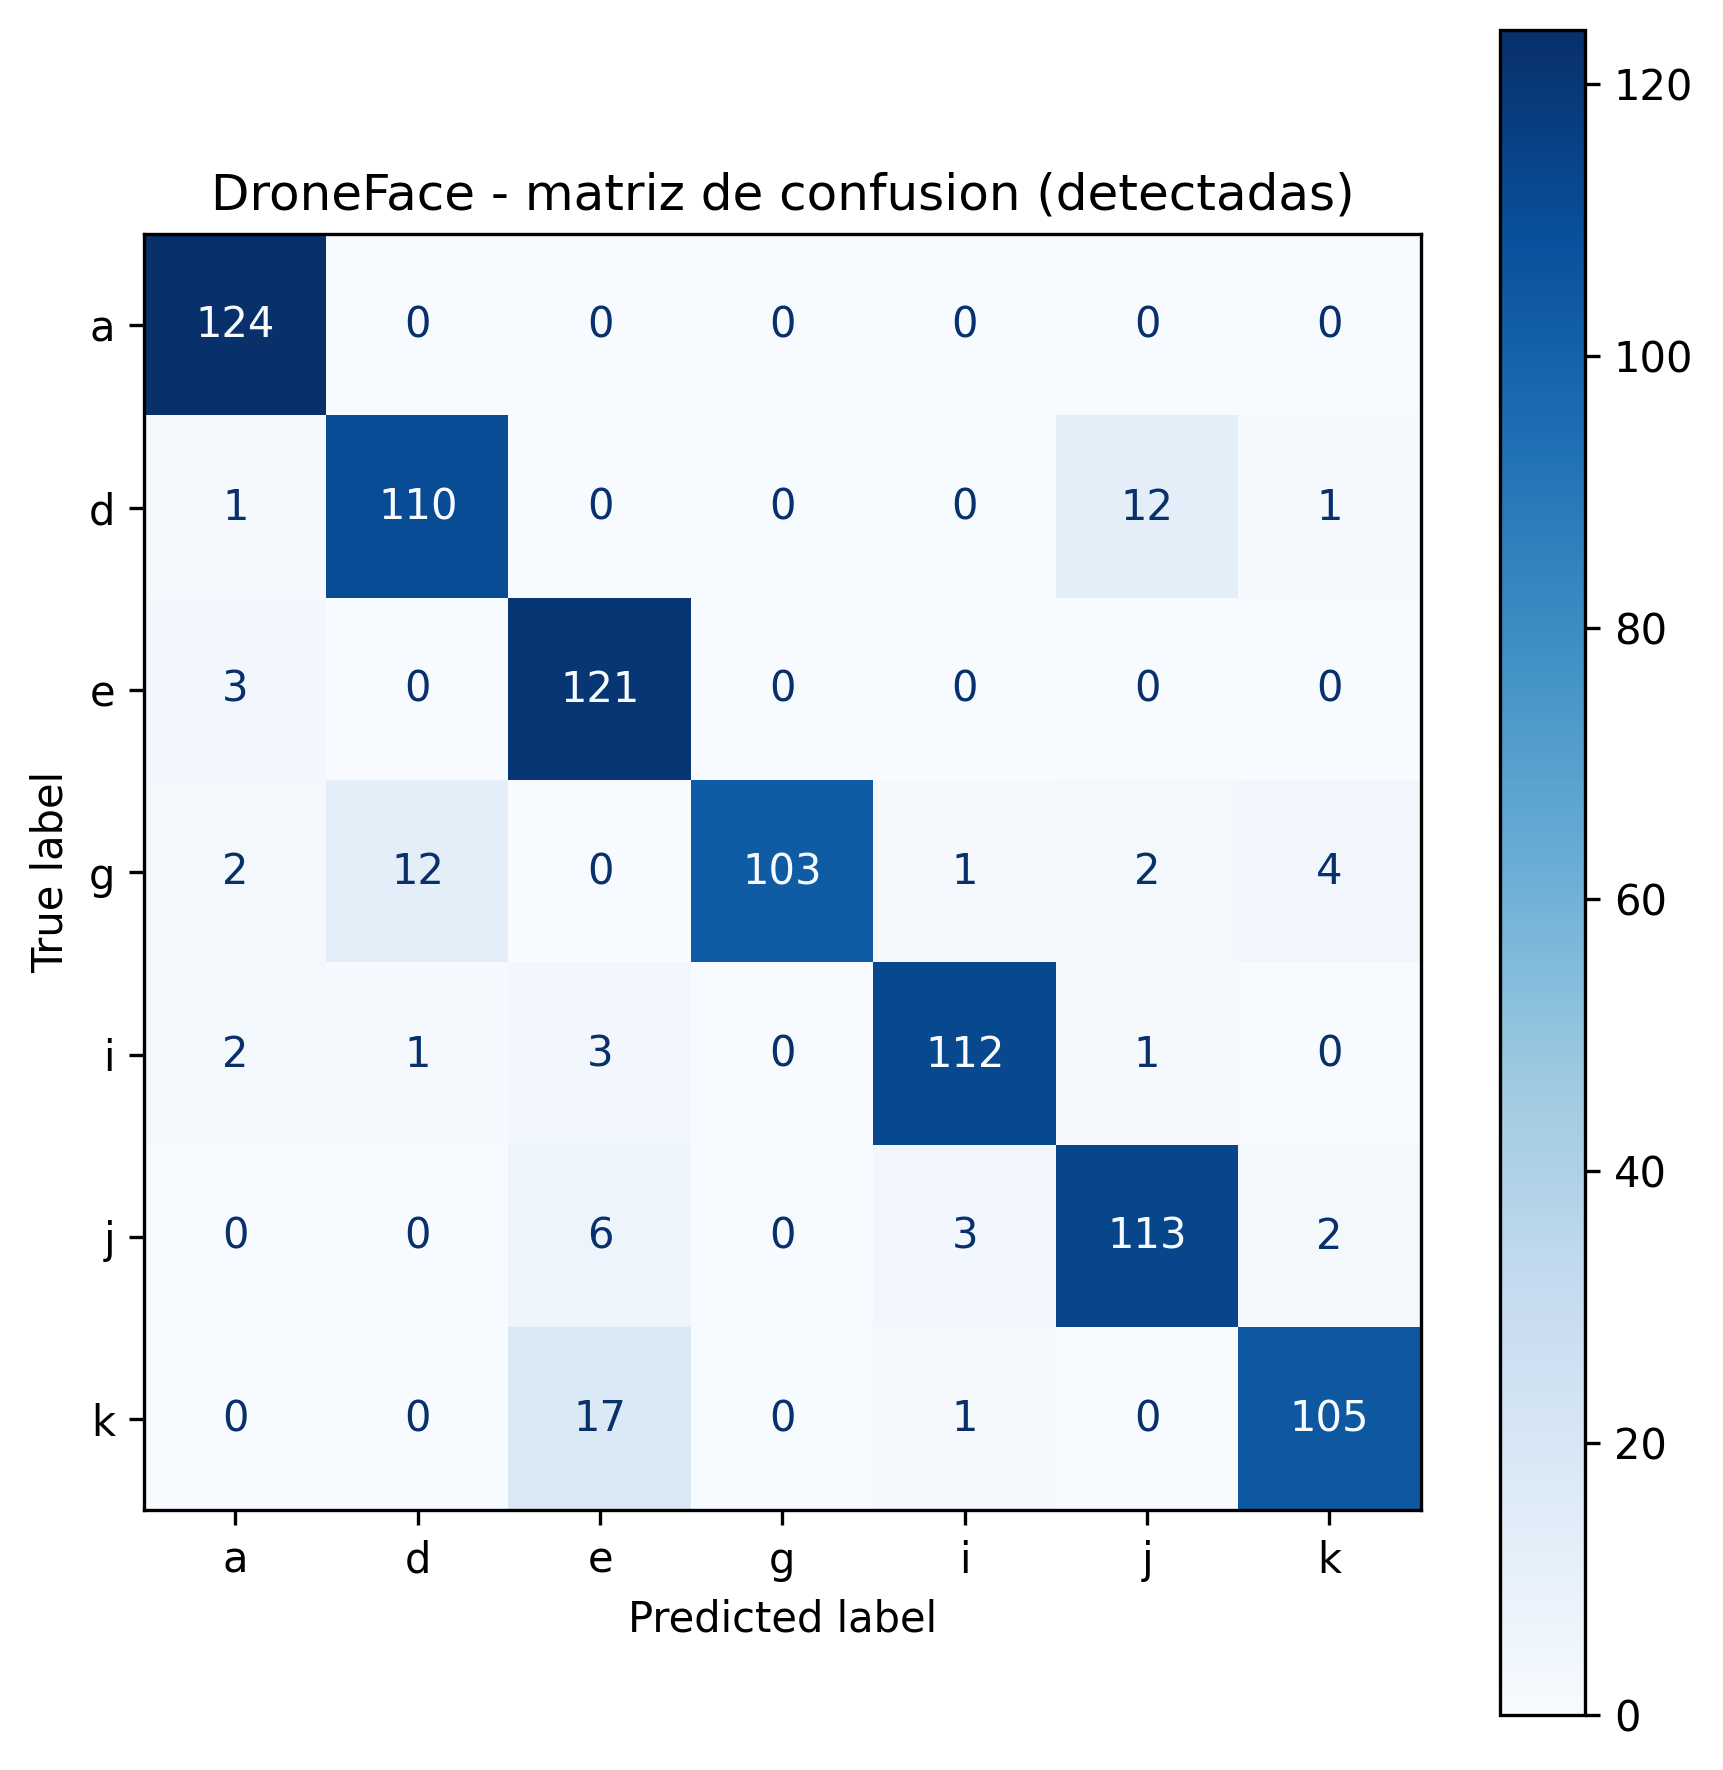
\includegraphics[width=0.9\textwidth]{metrics/droneface_confusion_matrix.png}
\caption{Matriz de confusión del Experimento A para sujetos con galería.}
\label{fig:confusion_a}
\end{figure}

\subsection{Experimento B}

La Tabla~\ref{tab:exp_b} resume el Experimento B. Se detectó al menos un rostro en 567 de 620 imágenes completas, lo que corresponde a una tasa de detección por imagen de 91.45\%. La recuperación global de identidades esperadas fue 78.80\%. Este resultado debe interpretarse como recuperación de identidades a nivel de imagen y no como reconocimiento correcto por crop, porque no existe una etiqueta de identidad asociada a cada caja detectada. Si una imagen contiene sujetos sin retrato de referencia, estos se registran como identidades esperadas sin galería y no se consideran dentro del denominador de recuperación.

\begin{table}[H]
\centering
\caption{Resultados del Experimento B con supervisión débil a nivel de imagen.}
\label{tab:exp_b}
\begin{tabular}{lc}
\toprule
Métrica & Valor \\
\midrule
Imágenes evaluadas & 620 \\
Imágenes con detección & 567 \\
\texttt{image\_detection\_rate} & 91.45\% \\
Identidades esperadas con galería & 868 \\
Identidades esperadas recuperadas & 684 \\
\texttt{expected\_identity\_recall\_global} & 78.80\% \\
\texttt{any\_expected\_found\_rate} & 84.19\% \\
\texttt{all\_expected\_found\_rate} & 77.58\% \\
\texttt{exact\_expected\_set\_match\_rate} & 25.48\% \\
\texttt{mean\_jaccard\_set\_similarity} & 54.10\% \\
Identidades inesperadas predichas & 399 \\
\bottomrule
\end{tabular}
\end{table}

En la Tabla~\ref{tab:exp_b}, la métrica \texttt{exact\_expected\_set\_match\_rate} es bastante más baja que \texttt{expected\_identity\_recall\_global}. Esto indica que el sistema suele recuperar parte importante de las identidades esperadas, pero no siempre recupera exactamente el conjunto completo sin identidades adicionales. La similitud de Jaccard complementa esta lectura al medir el solapamiento entre el conjunto esperado y el conjunto predicho.

\begin{figure}[H]
\centering
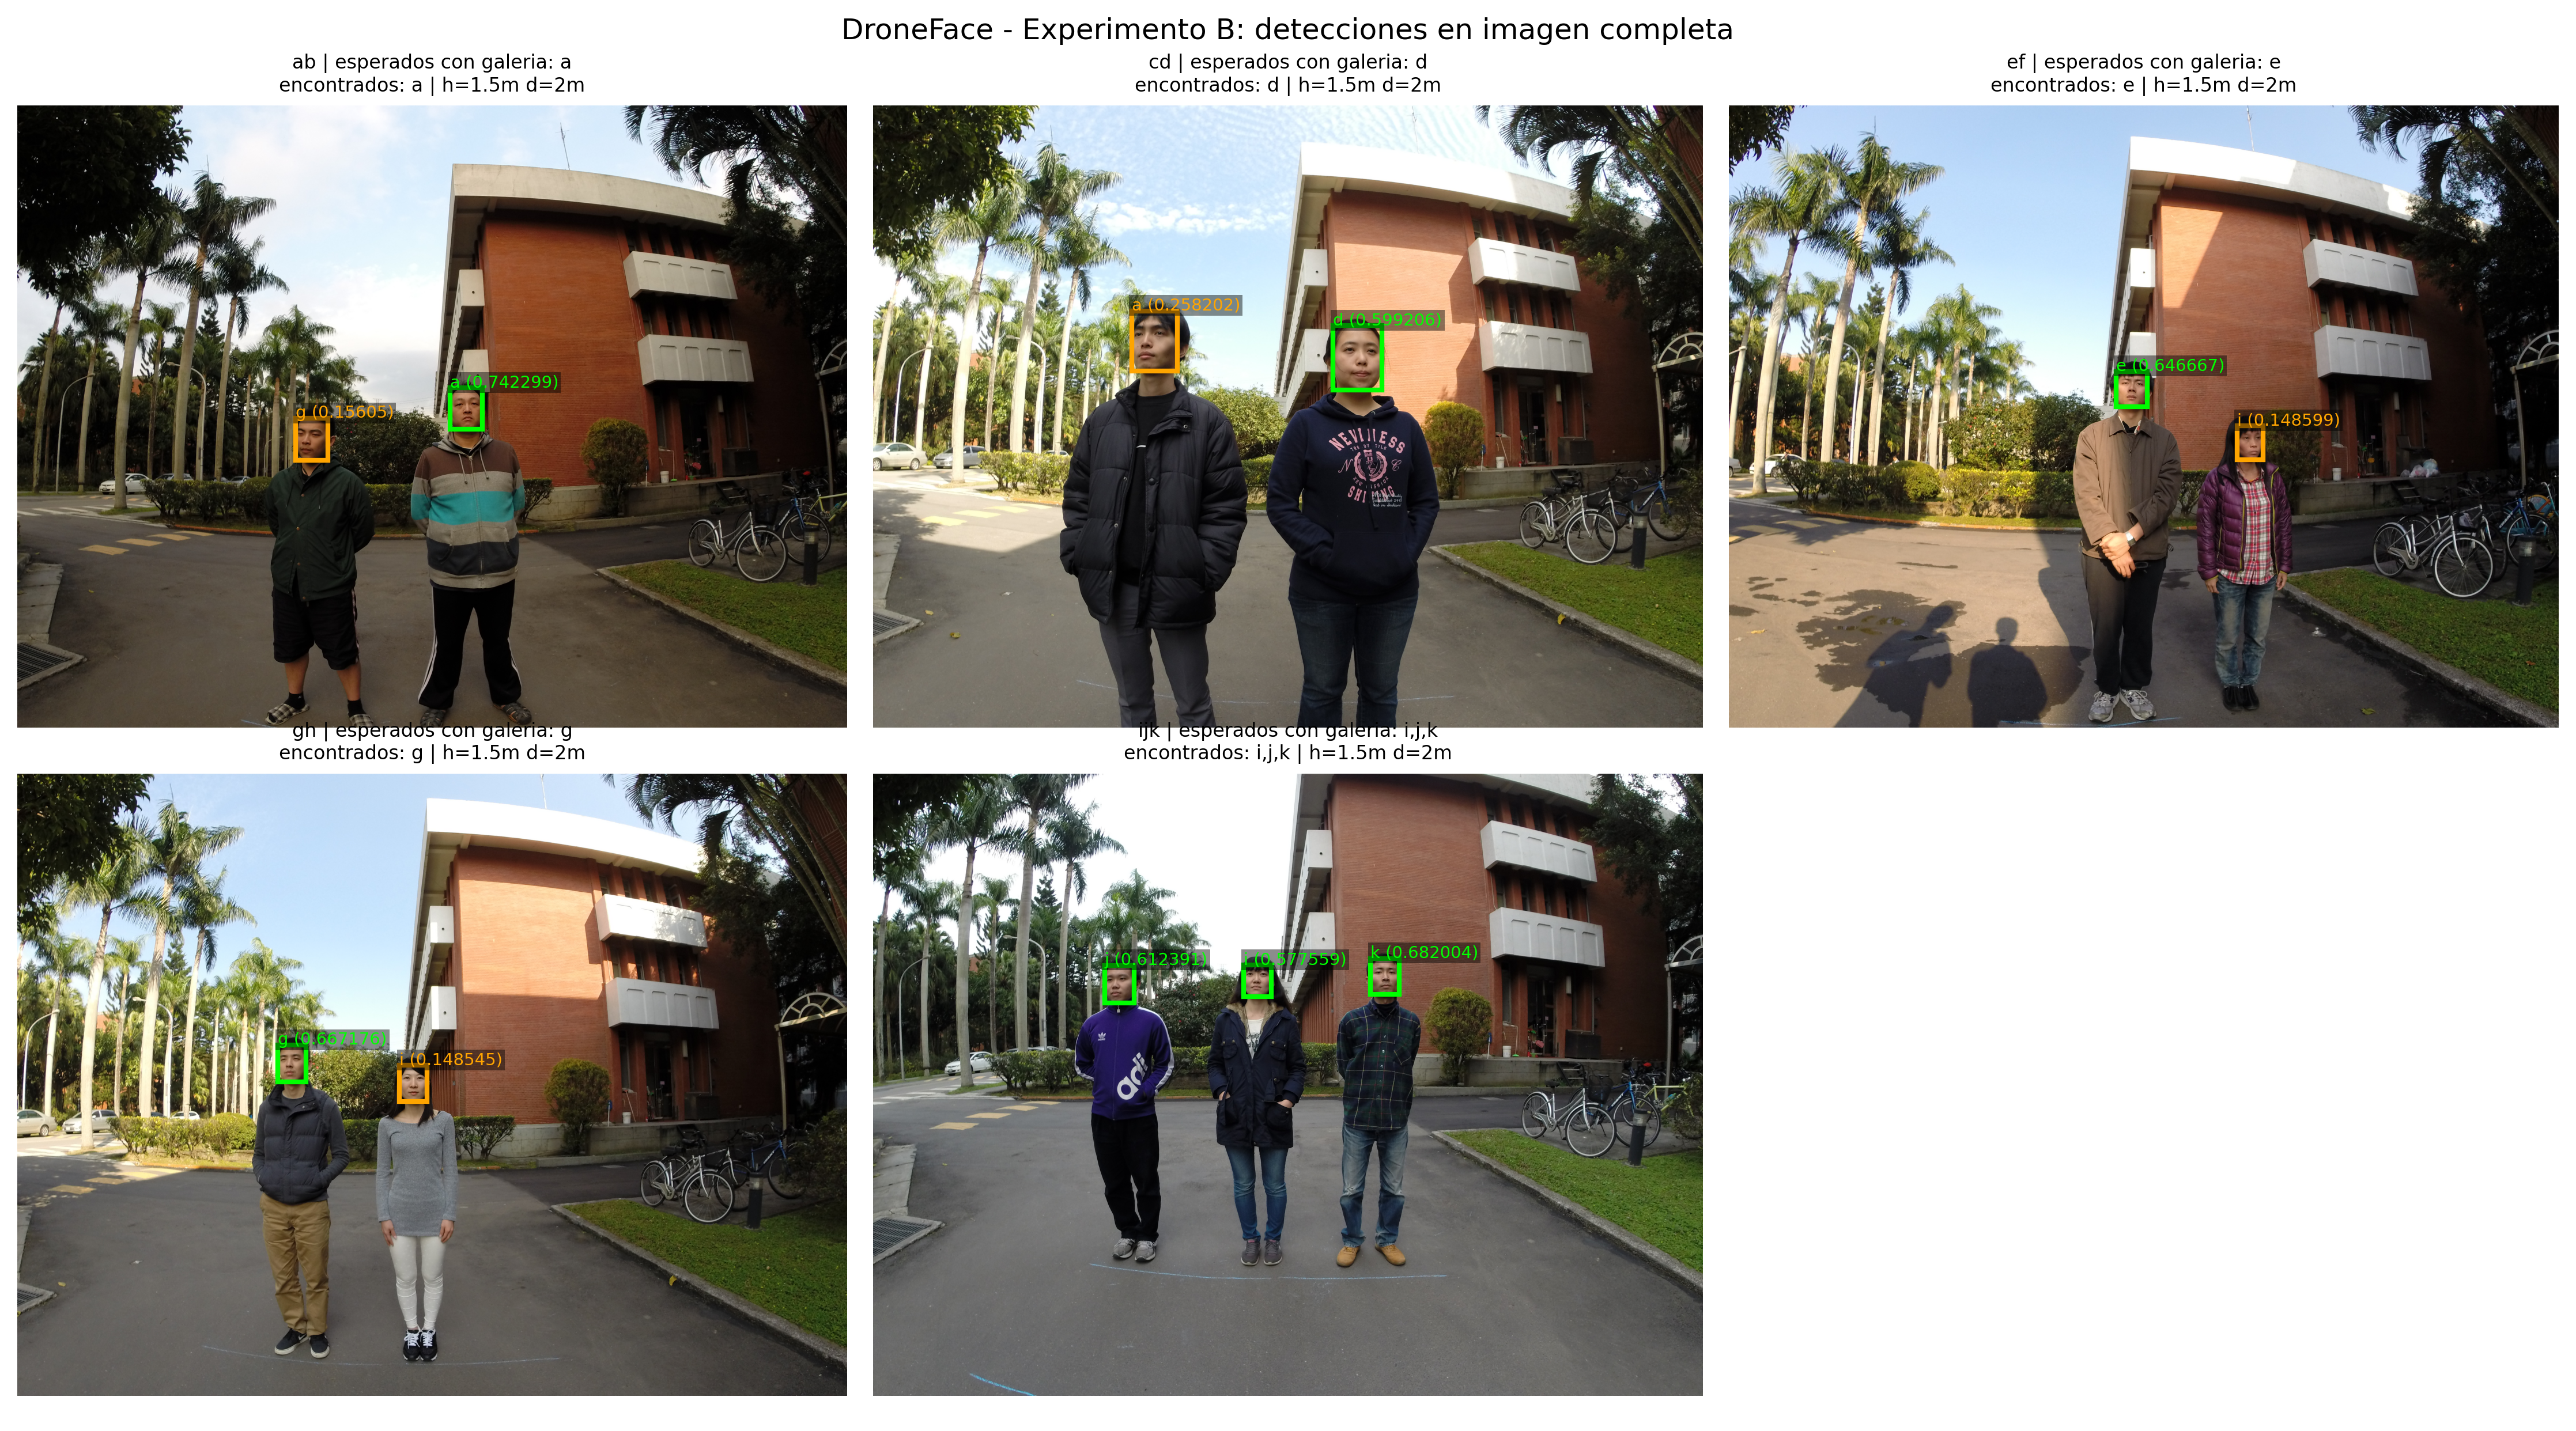
\includegraphics[width=0.85\textwidth]{detection/droneface_full_image_detections.png}
\caption{Ejemplos del Experimento B. Las cajas provienen de detecciones en la imagen completa; las etiquetas indican identidades predichas por similitud con la galería.}
\label{fig:full_detections}
\end{figure}

La Figura~\ref{fig:full_detections} muestra ejemplos del flujo completo: primero se detectan rostros en la imagen de dron y luego cada detección se compara contra la galería. Estas visualizaciones son útiles para auditar el comportamiento, pero no reemplazan una anotación manual por bounding box.

\begin{figure}[H]
\centering
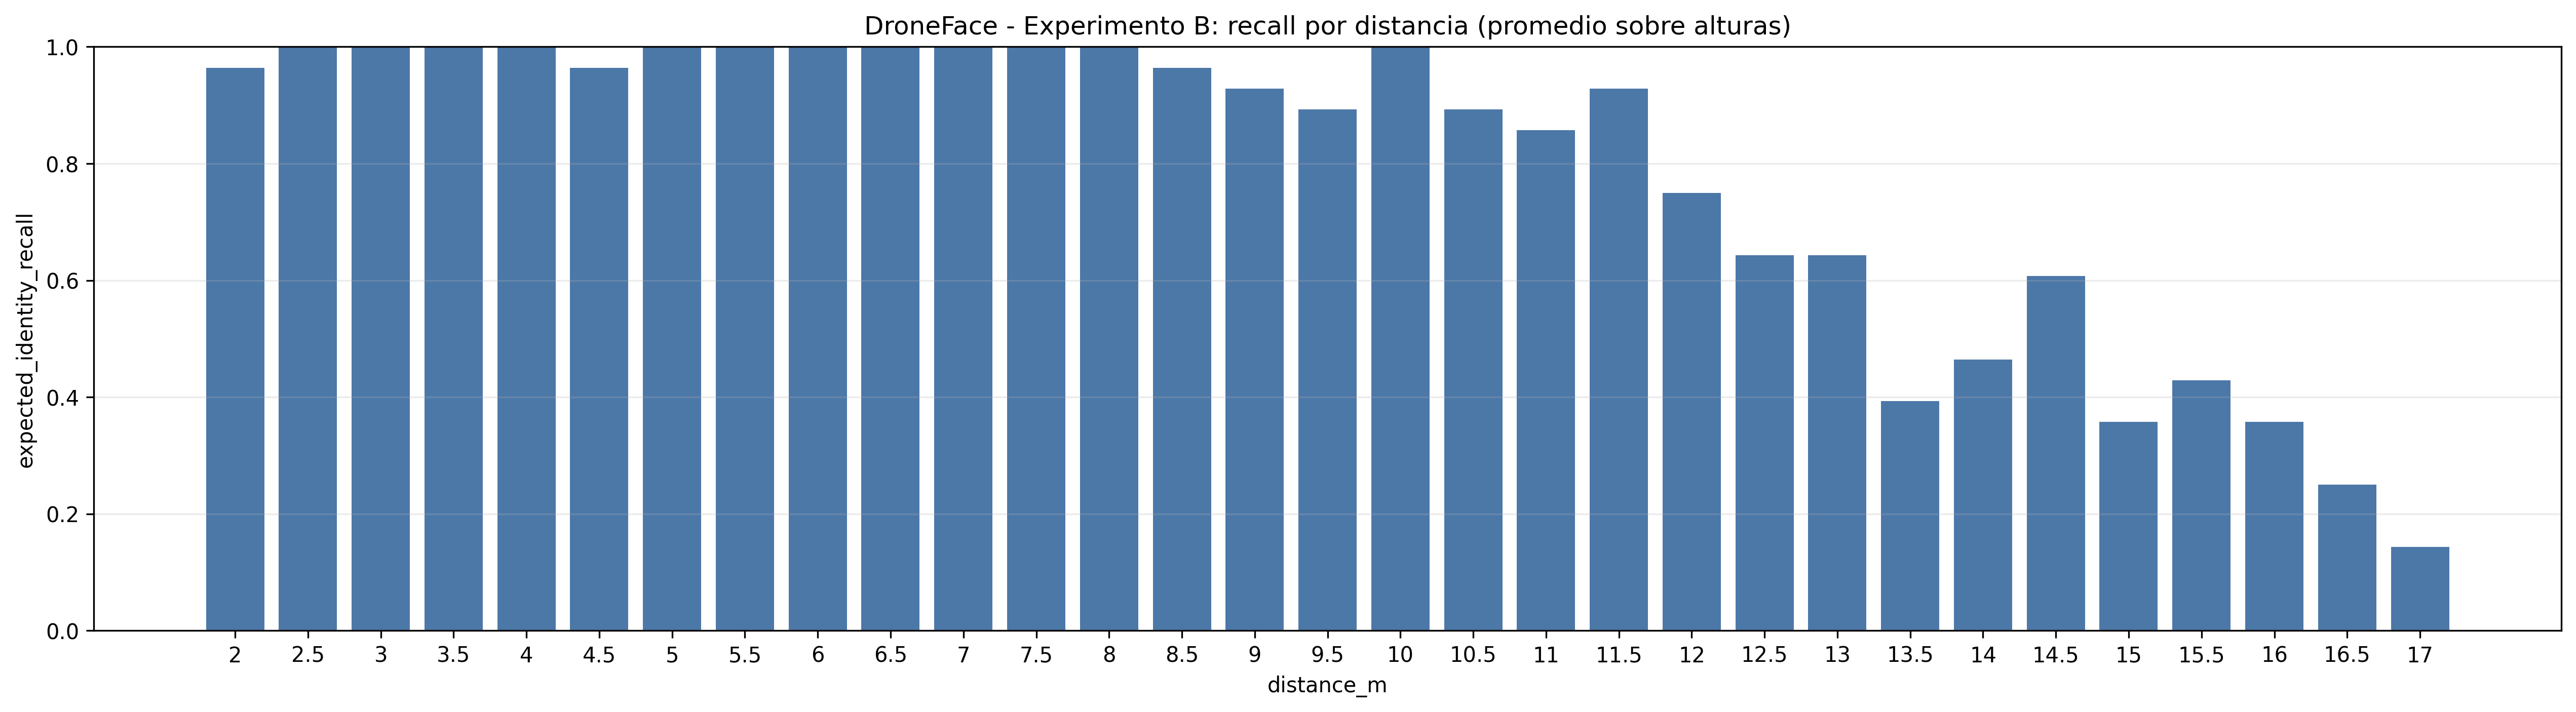
\includegraphics[width=0.95\textwidth]{metrics/droneface_full_image_recall_by_distance.png}
\caption{Recuperación de identidades esperadas del Experimento B por distancia.}
\label{fig:exp_b_distancia}
\end{figure}

En la Figura~\ref{fig:exp_b_distancia} se observa una caída clara a distancias altas. La comparación con el Experimento A en la Figura~\ref{fig:exp_ab_comparacion} muestra que el flujo de imagen completa es más difícil que evaluar rostros ya recortados, porque combina detección de rostros pequeños, alineamiento y reconocimiento.

\begin{figure}[H]
\centering
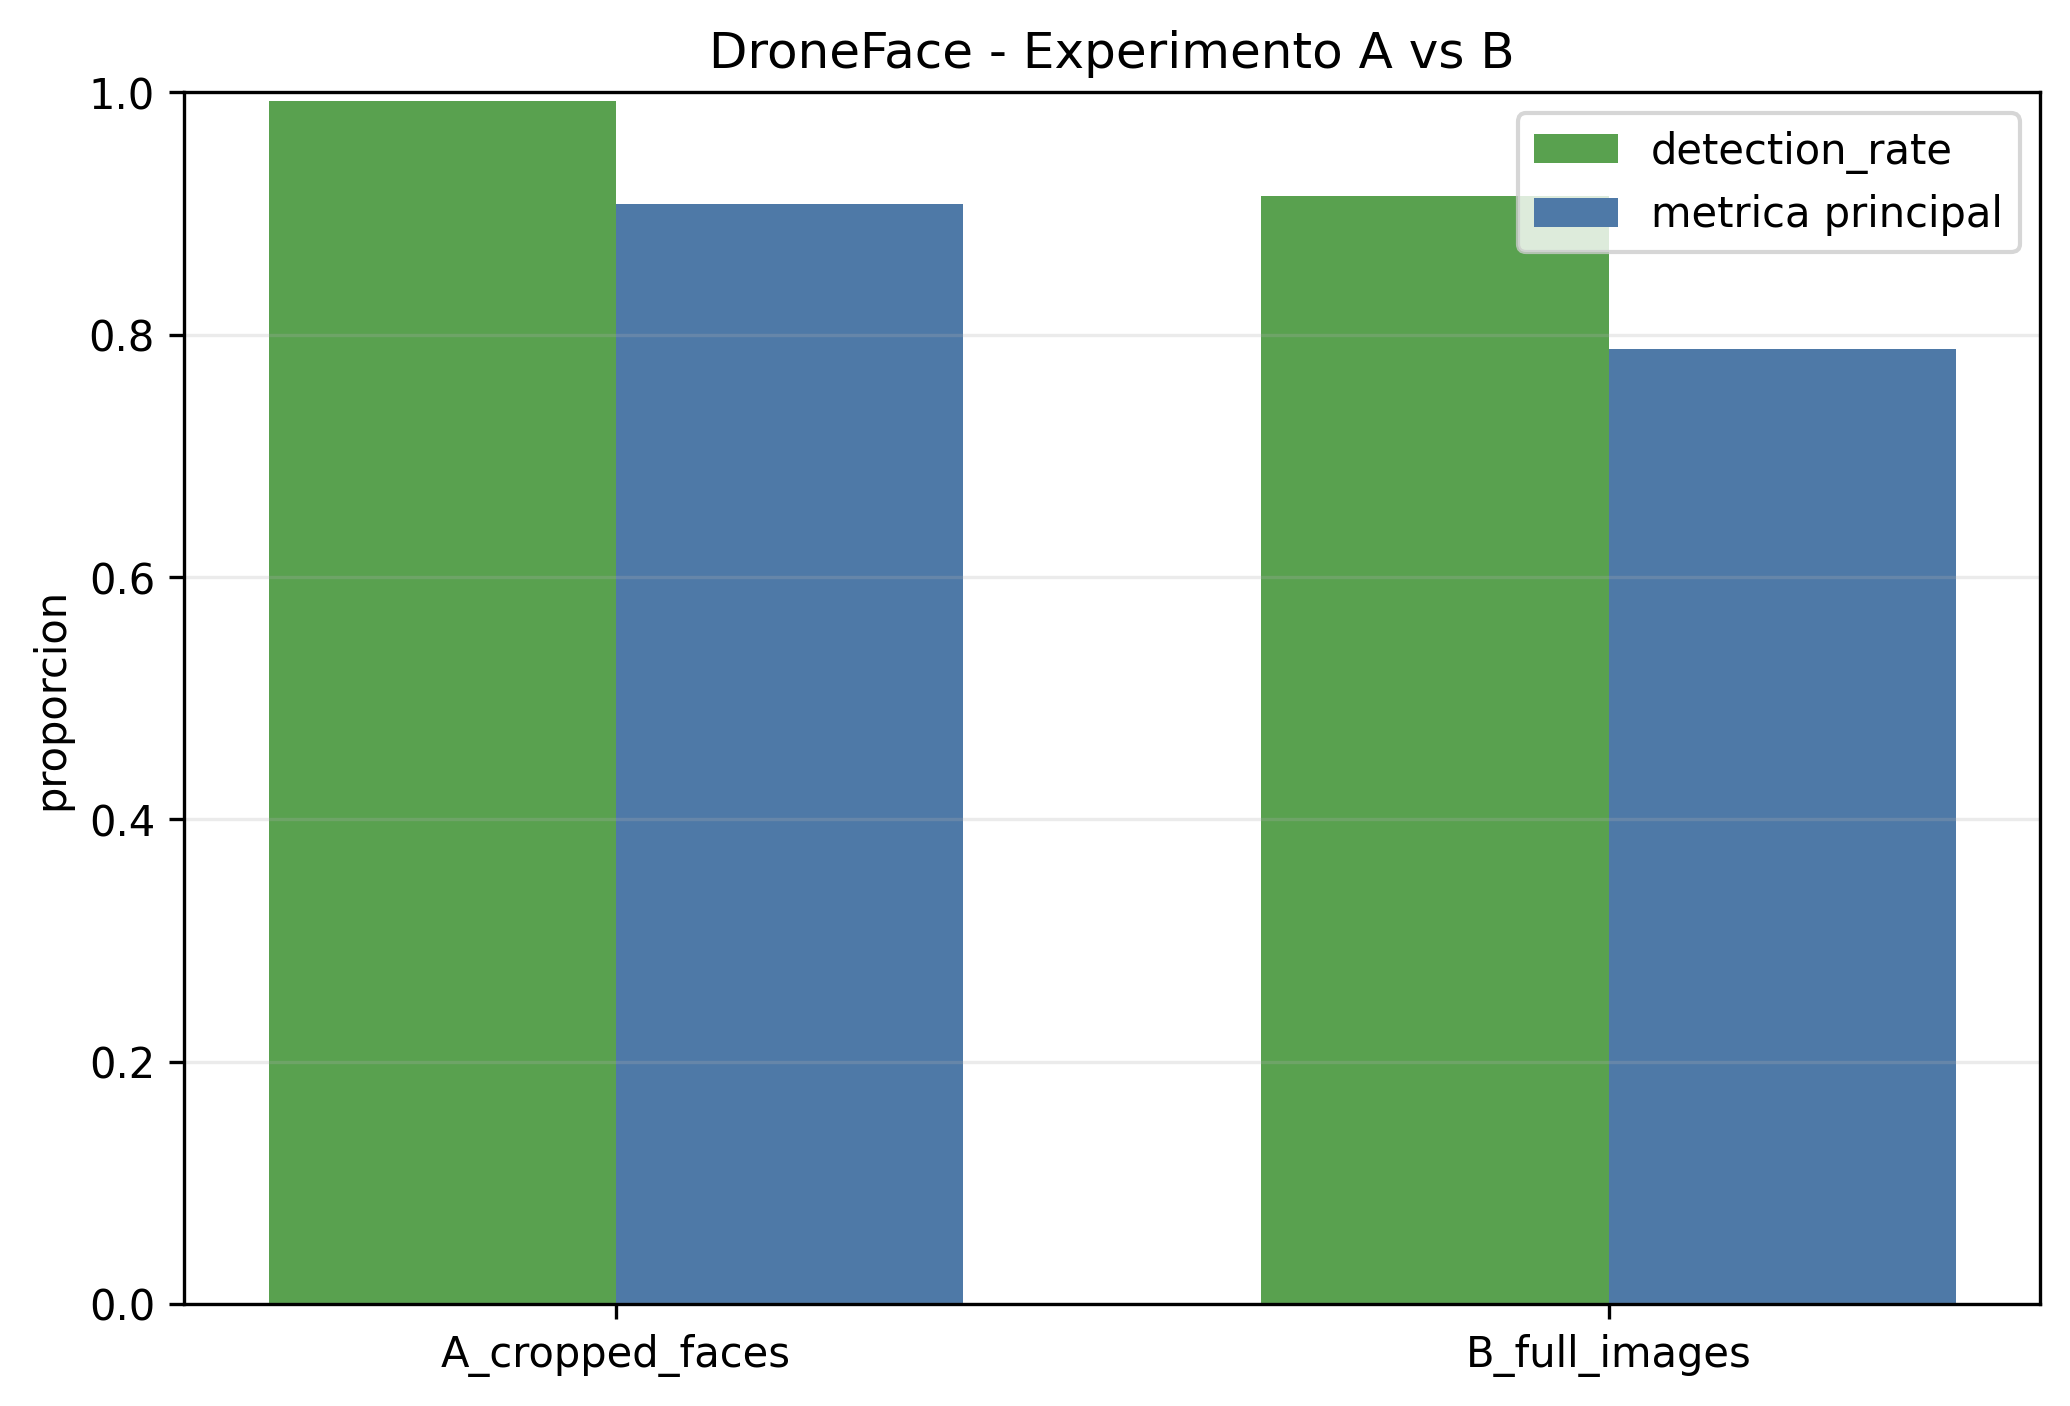
\includegraphics[width=0.88\textwidth]{metrics/droneface_experiment_a_vs_b.png}
\caption{Comparación entre la métrica principal del Experimento A y la recuperación de identidades esperadas del Experimento B.}
\label{fig:exp_ab_comparacion}
\end{figure}

La Figura~\ref{fig:heatmap_b} muestra el mismo fenómeno por altura y distancia. Las zonas con menor recuperación corresponden a condiciones donde los rostros son más pequeños o menos definidos, lo que afecta principalmente la detección inicial.

\begin{figure}[H]
\centering
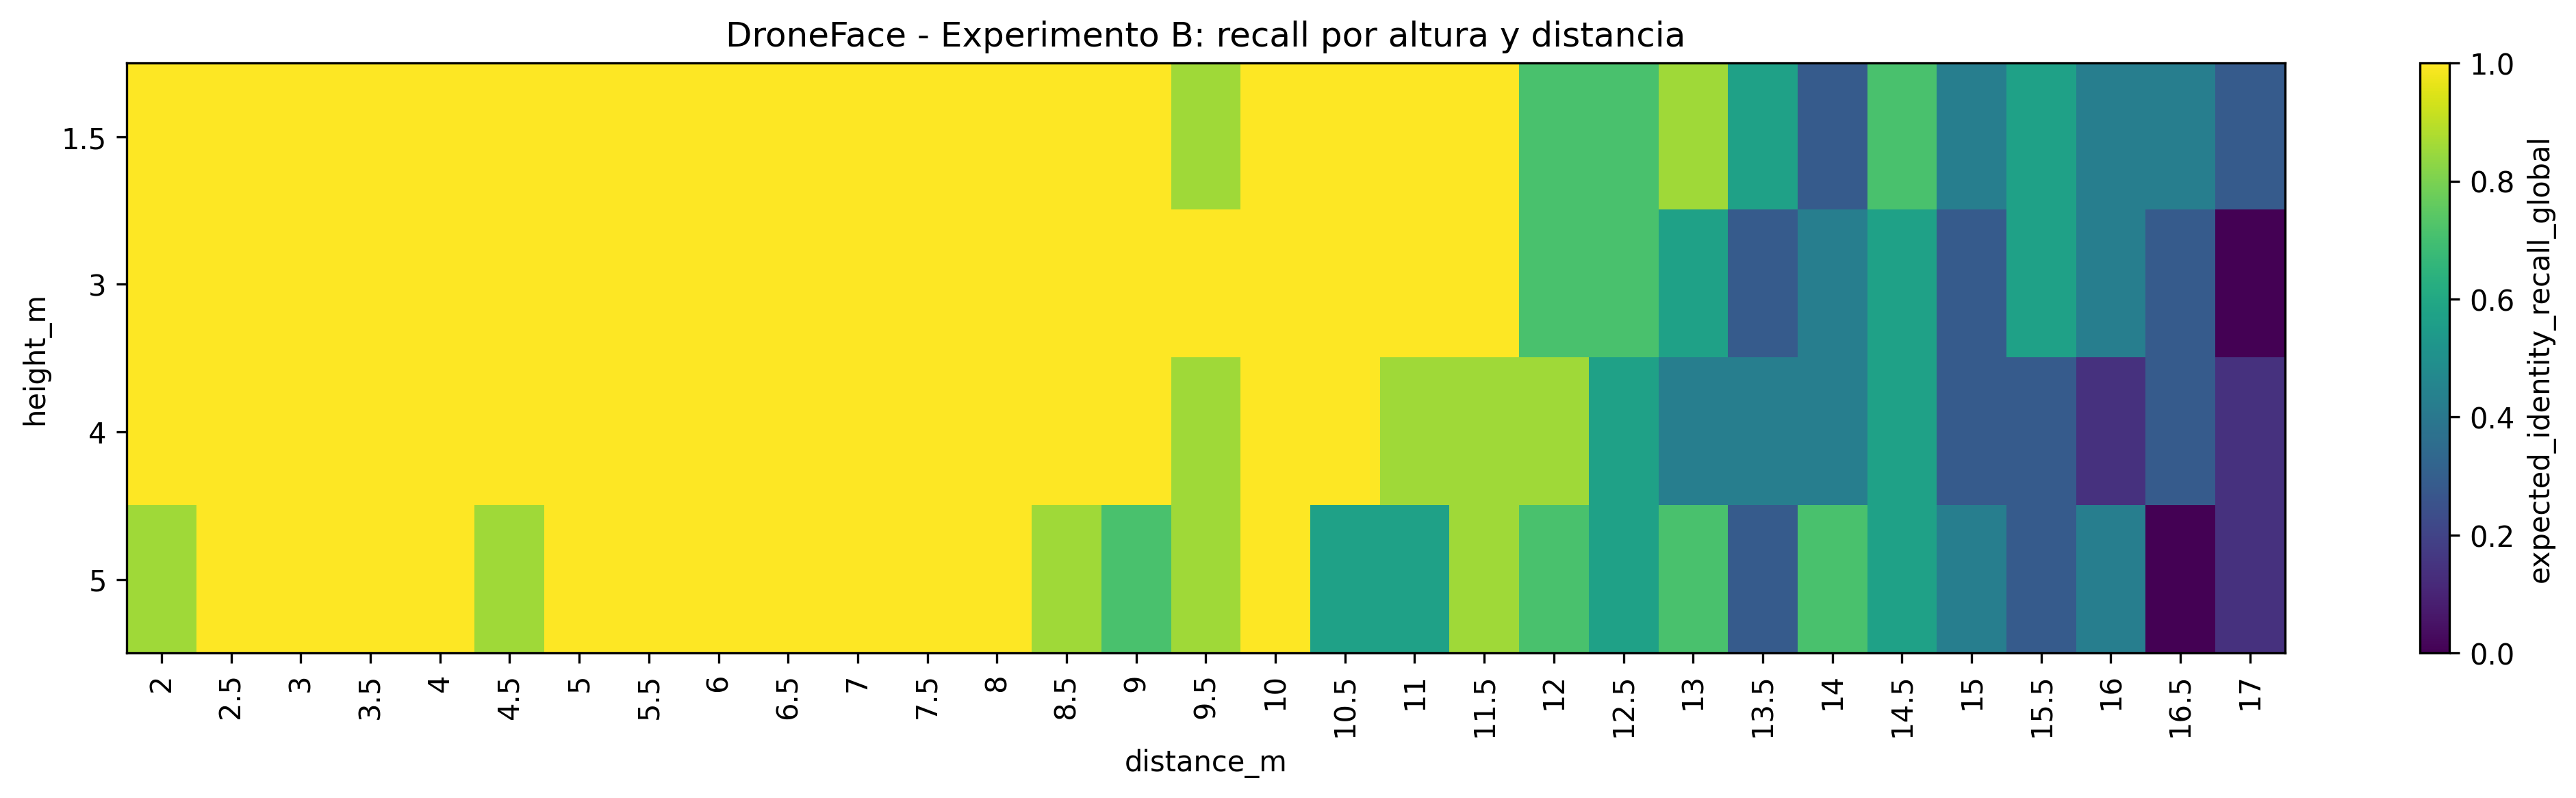
\includegraphics[width=\textwidth]{metrics/droneface_full_image_recall_height_distance.png}
\caption{Mapa de calor de recuperación de identidades esperadas en el Experimento B.}
\label{fig:heatmap_b}
\end{figure}

Además, se evaluó la sensibilidad al parámetro \texttt{det\_size} en imágenes completas. A mayor \texttt{det\_size}, el detector trabaja con una entrada más grande y logra recuperar más rostros pequeños, aunque con mayor costo computacional. La Tabla~\ref{tab:det_size_b} y la Figura~\ref{fig:det_size_b} muestran que \texttt{det\_size=1280} fue la mejor configuración probada para B, tanto en tasa de detección por imagen como en recuperación global de identidades esperadas.

\begin{table}[H]
\centering
\caption{Barrido de \texttt{det\_size} para el Experimento B.}
\label{tab:det_size_b}
\begin{tabular}{ccc}
\toprule
\texttt{det\_size} & \texttt{image\_detection\_rate} & \texttt{expected\_identity\_recall\_global} \\
\midrule
320 & 9.03\% & 6.68\% \\
640 & 41.13\% & 33.29\% \\
1024 & 75.32\% & 63.82\% \\
1280 & 91.45\% & 78.80\% \\
\bottomrule
\end{tabular}
\end{table}

\begin{figure}[H]
\centering
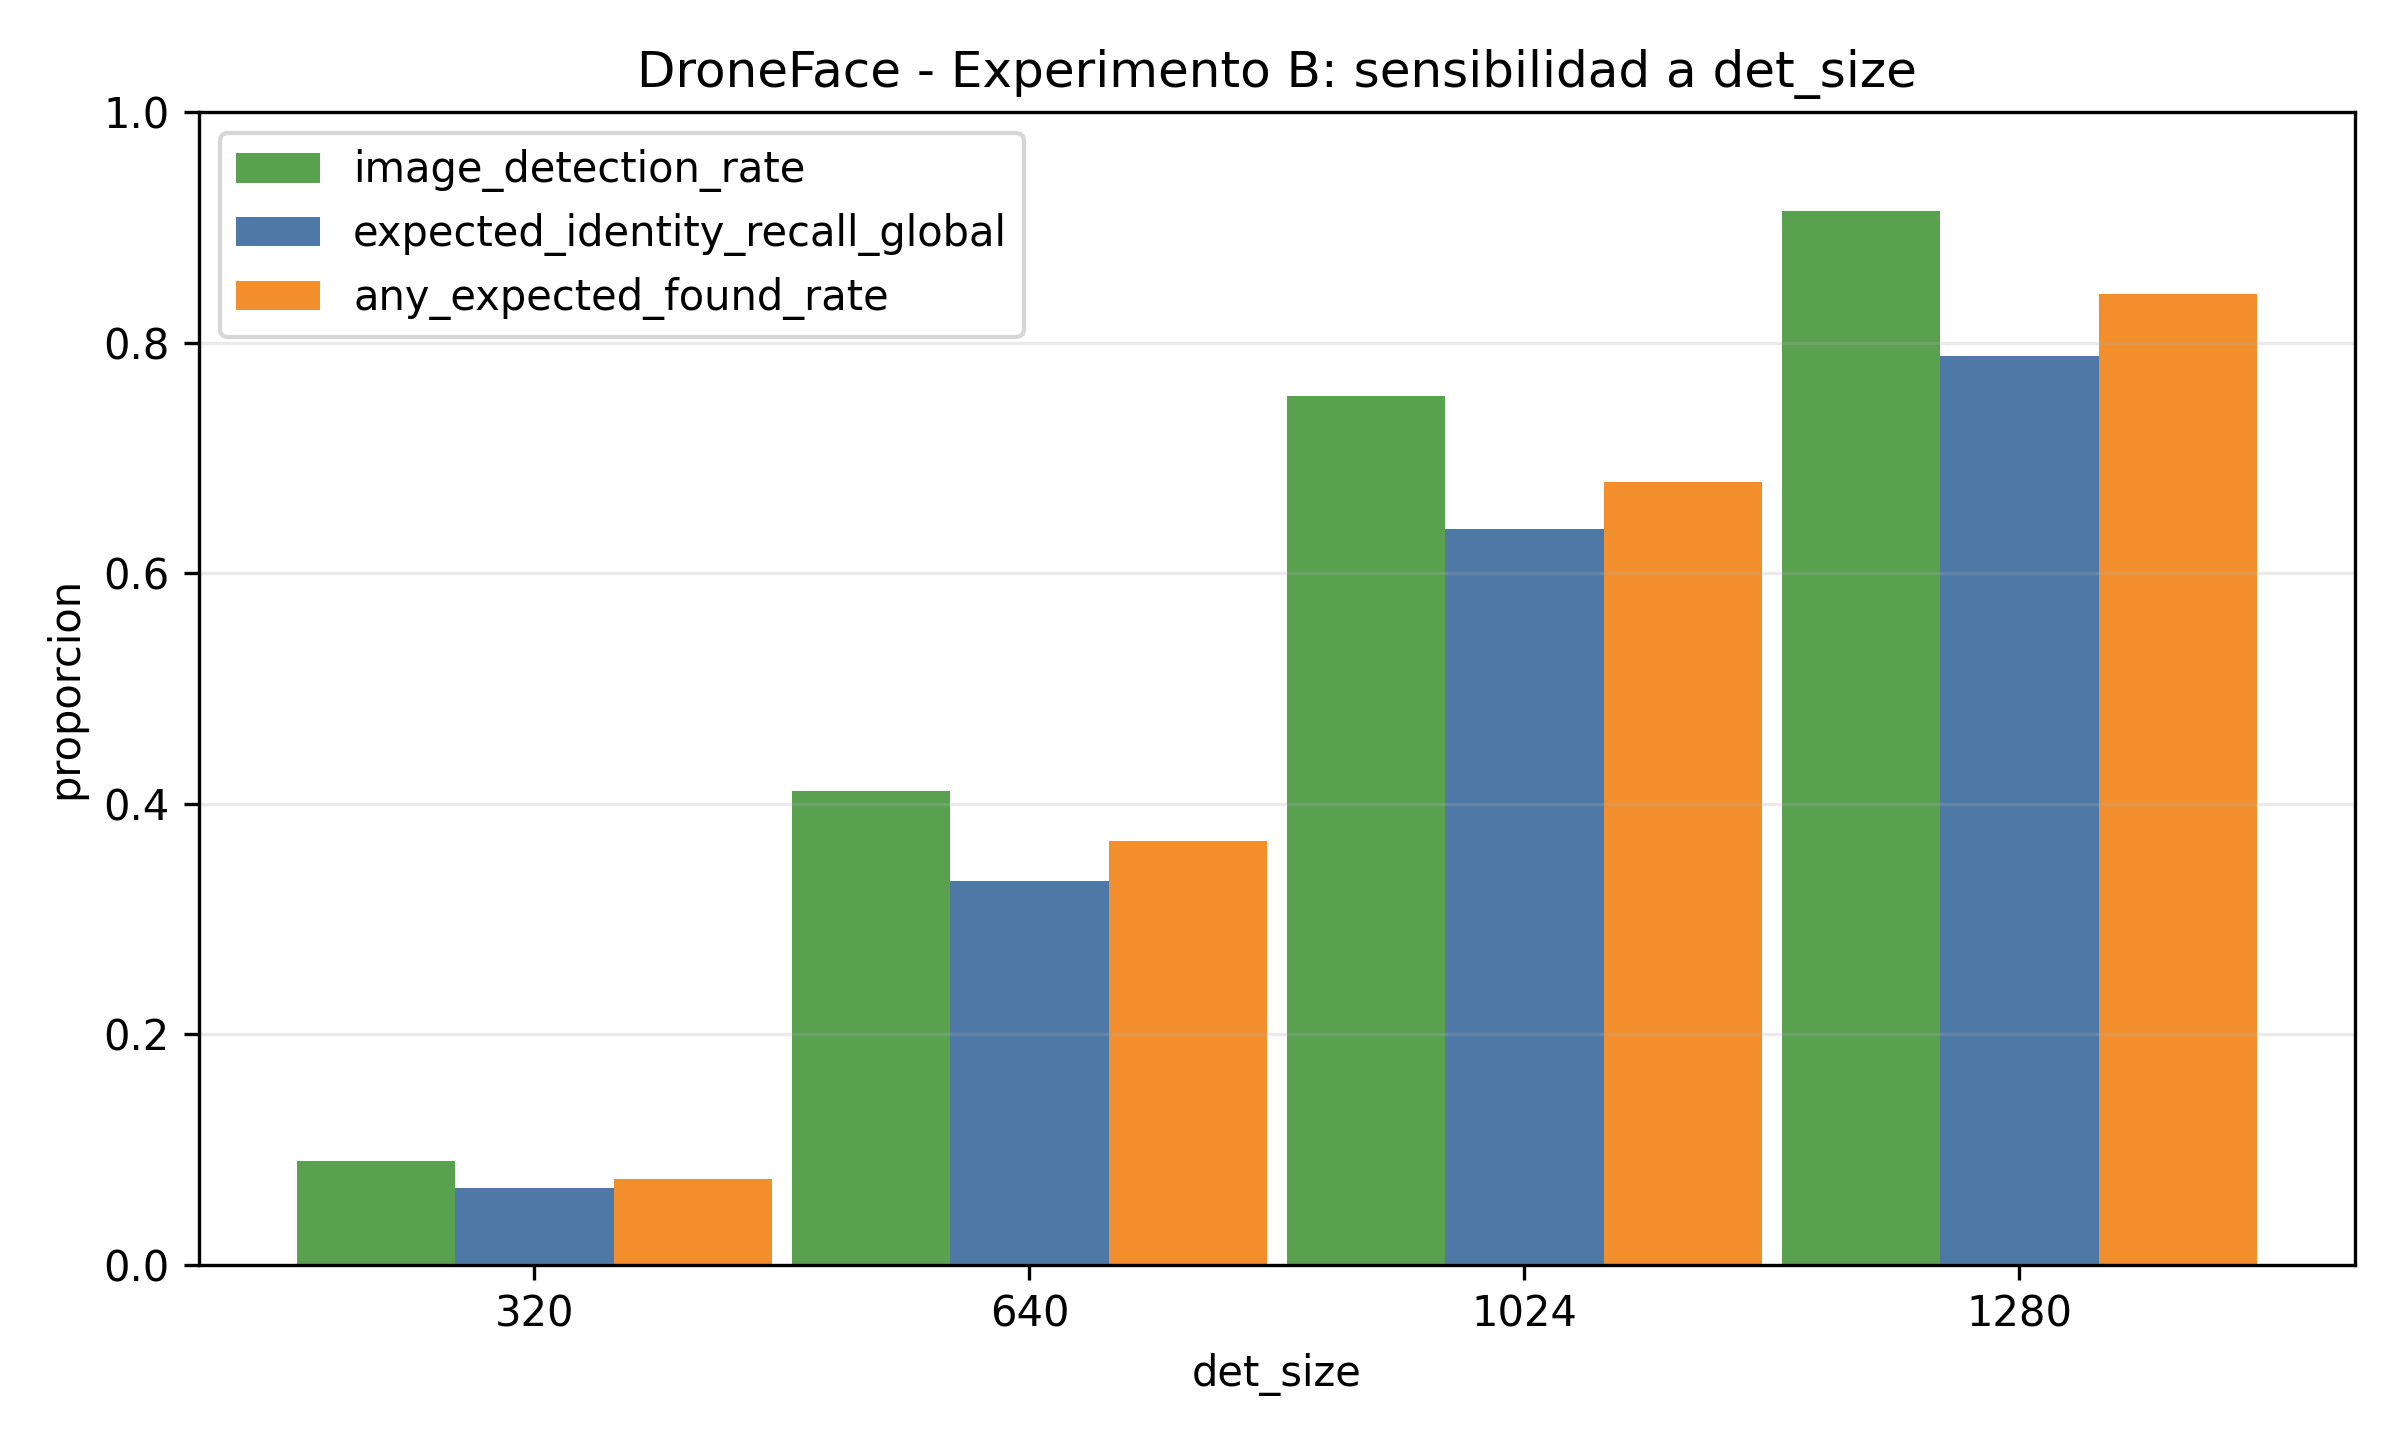
\includegraphics[width=0.95\textwidth]{metrics/droneface_full_image_det_size_sweep.png}
\caption{Barrido de \texttt{det\_size} en imágenes completas del Experimento B.}
\label{fig:det_size_b}
\end{figure}

\subsection{Experimento C}

La Tabla~\ref{tab:exp_c} muestra cómo cae el reconocimiento cuando se degradan artificialmente probes con identidad conocida. En la referencia limpia se obtiene 100\% de \rankone, porque los probes fueron seleccionados desde casos que el Experimento A ya reconocía correctamente. A medida que aumenta la degradación, el desempeño disminuye de forma gradual.

\begin{table}[H]
\centering
\caption{Resultados del Experimento C con degradación sintética.}
\label{tab:exp_c}
\begin{adjustbox}{max width=\textwidth}
\begin{tabular}{lccc}
\toprule
Nivel & \texttt{detection\_rate} & \texttt{rank1\_accuracy\_conditional} & \texttt{rank1\_accuracy\_global} \\
\midrule
\texttt{clean\_reference} & 100.00\% & 100.00\% & 100.00\% \\
\texttt{mild} & 99.52\% & 94.74\% & 94.29\% \\
\texttt{medium} & 98.10\% & 87.38\% & 85.71\% \\
\texttt{strong} & 96.19\% & 77.23\% & 74.29\% \\
\bottomrule
\end{tabular}
\end{adjustbox}
\end{table}

La Figura~\ref{fig:exp_c_rank1} permite leer la tendencia: la detección baja poco, desde 100.00\% hasta 96.19\%, mientras que el \rankone{} global cae con más fuerza, desde 100.00\% hasta 74.29\%. Por lo tanto, bajo degradación fuerte el error no se explica solo por pérdida de detecciones, sino también por embeddings menos discriminativos.

\begin{figure}[H]
\centering
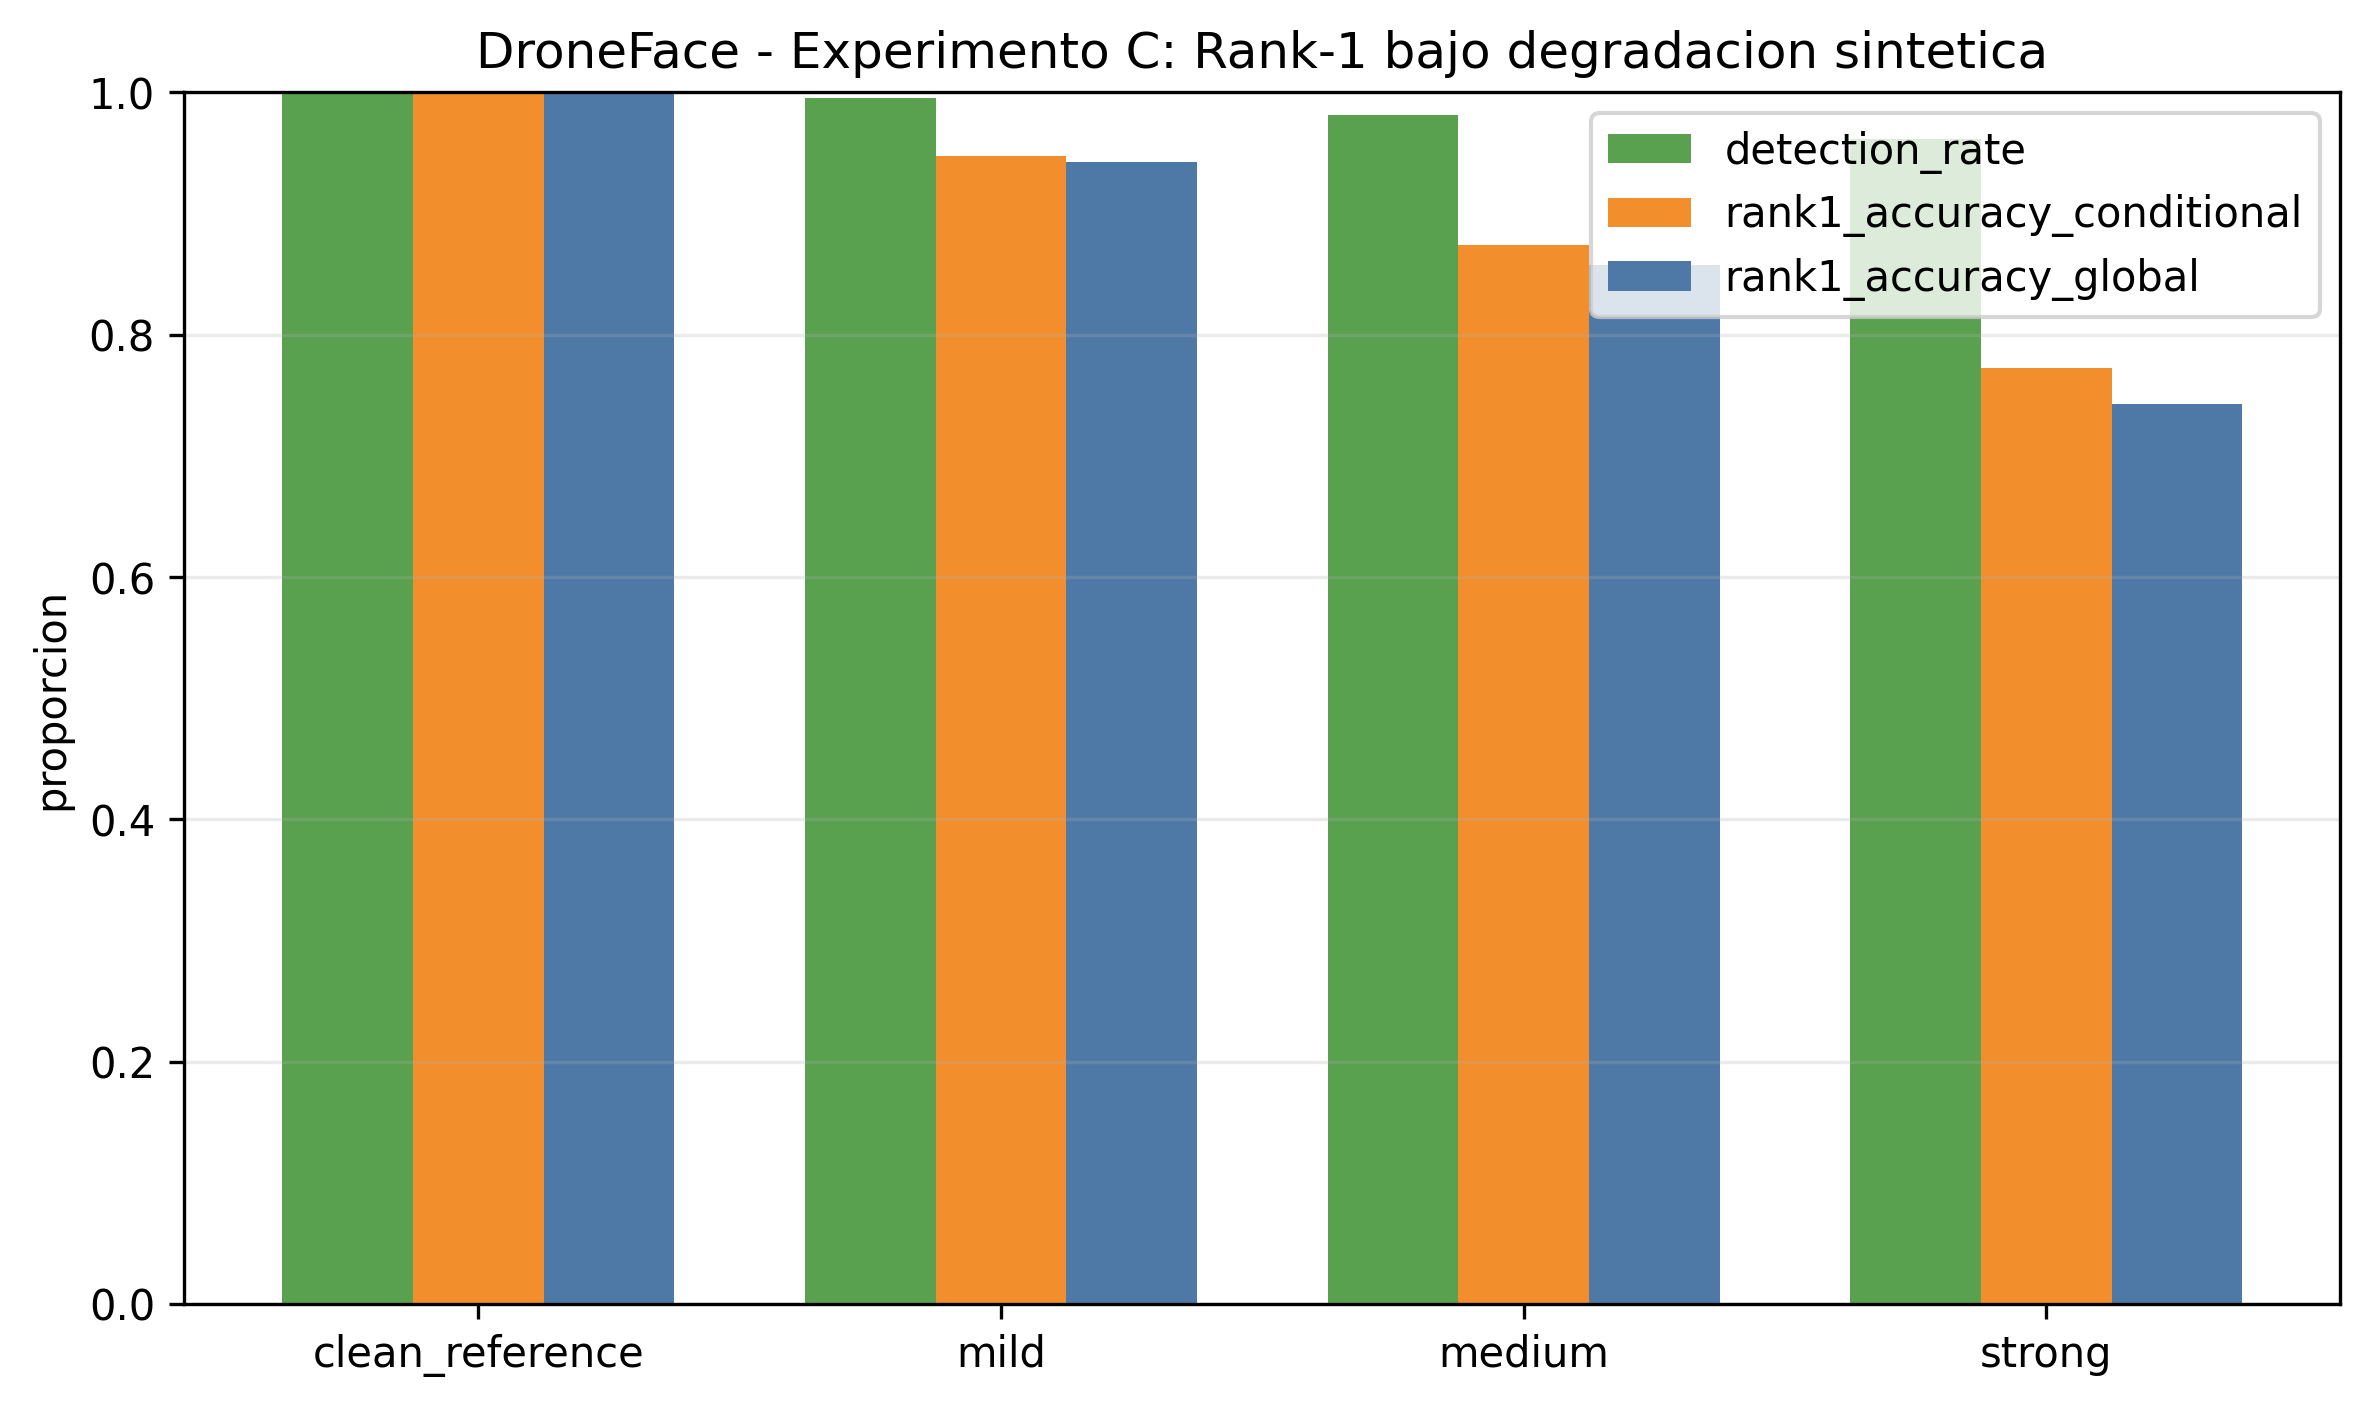
\includegraphics[width=0.95\textwidth]{metrics/droneface_synthetic_degradation_rank1.png}
\caption{Evolución de la detección y del \rankone{} bajo degradación sintética.}
\label{fig:exp_c_rank1}
\end{figure}

La Figura~\ref{fig:exp_c_examples} muestra ejemplos visuales del protocolo sintético. Esta figura justifica cualitativamente que las degradaciones simuladas son relevantes para imágenes de dron: reducen detalle facial, agregan blur y deterioran la compresión sin cambiar la identidad real.

\begin{figure}[H]
\centering
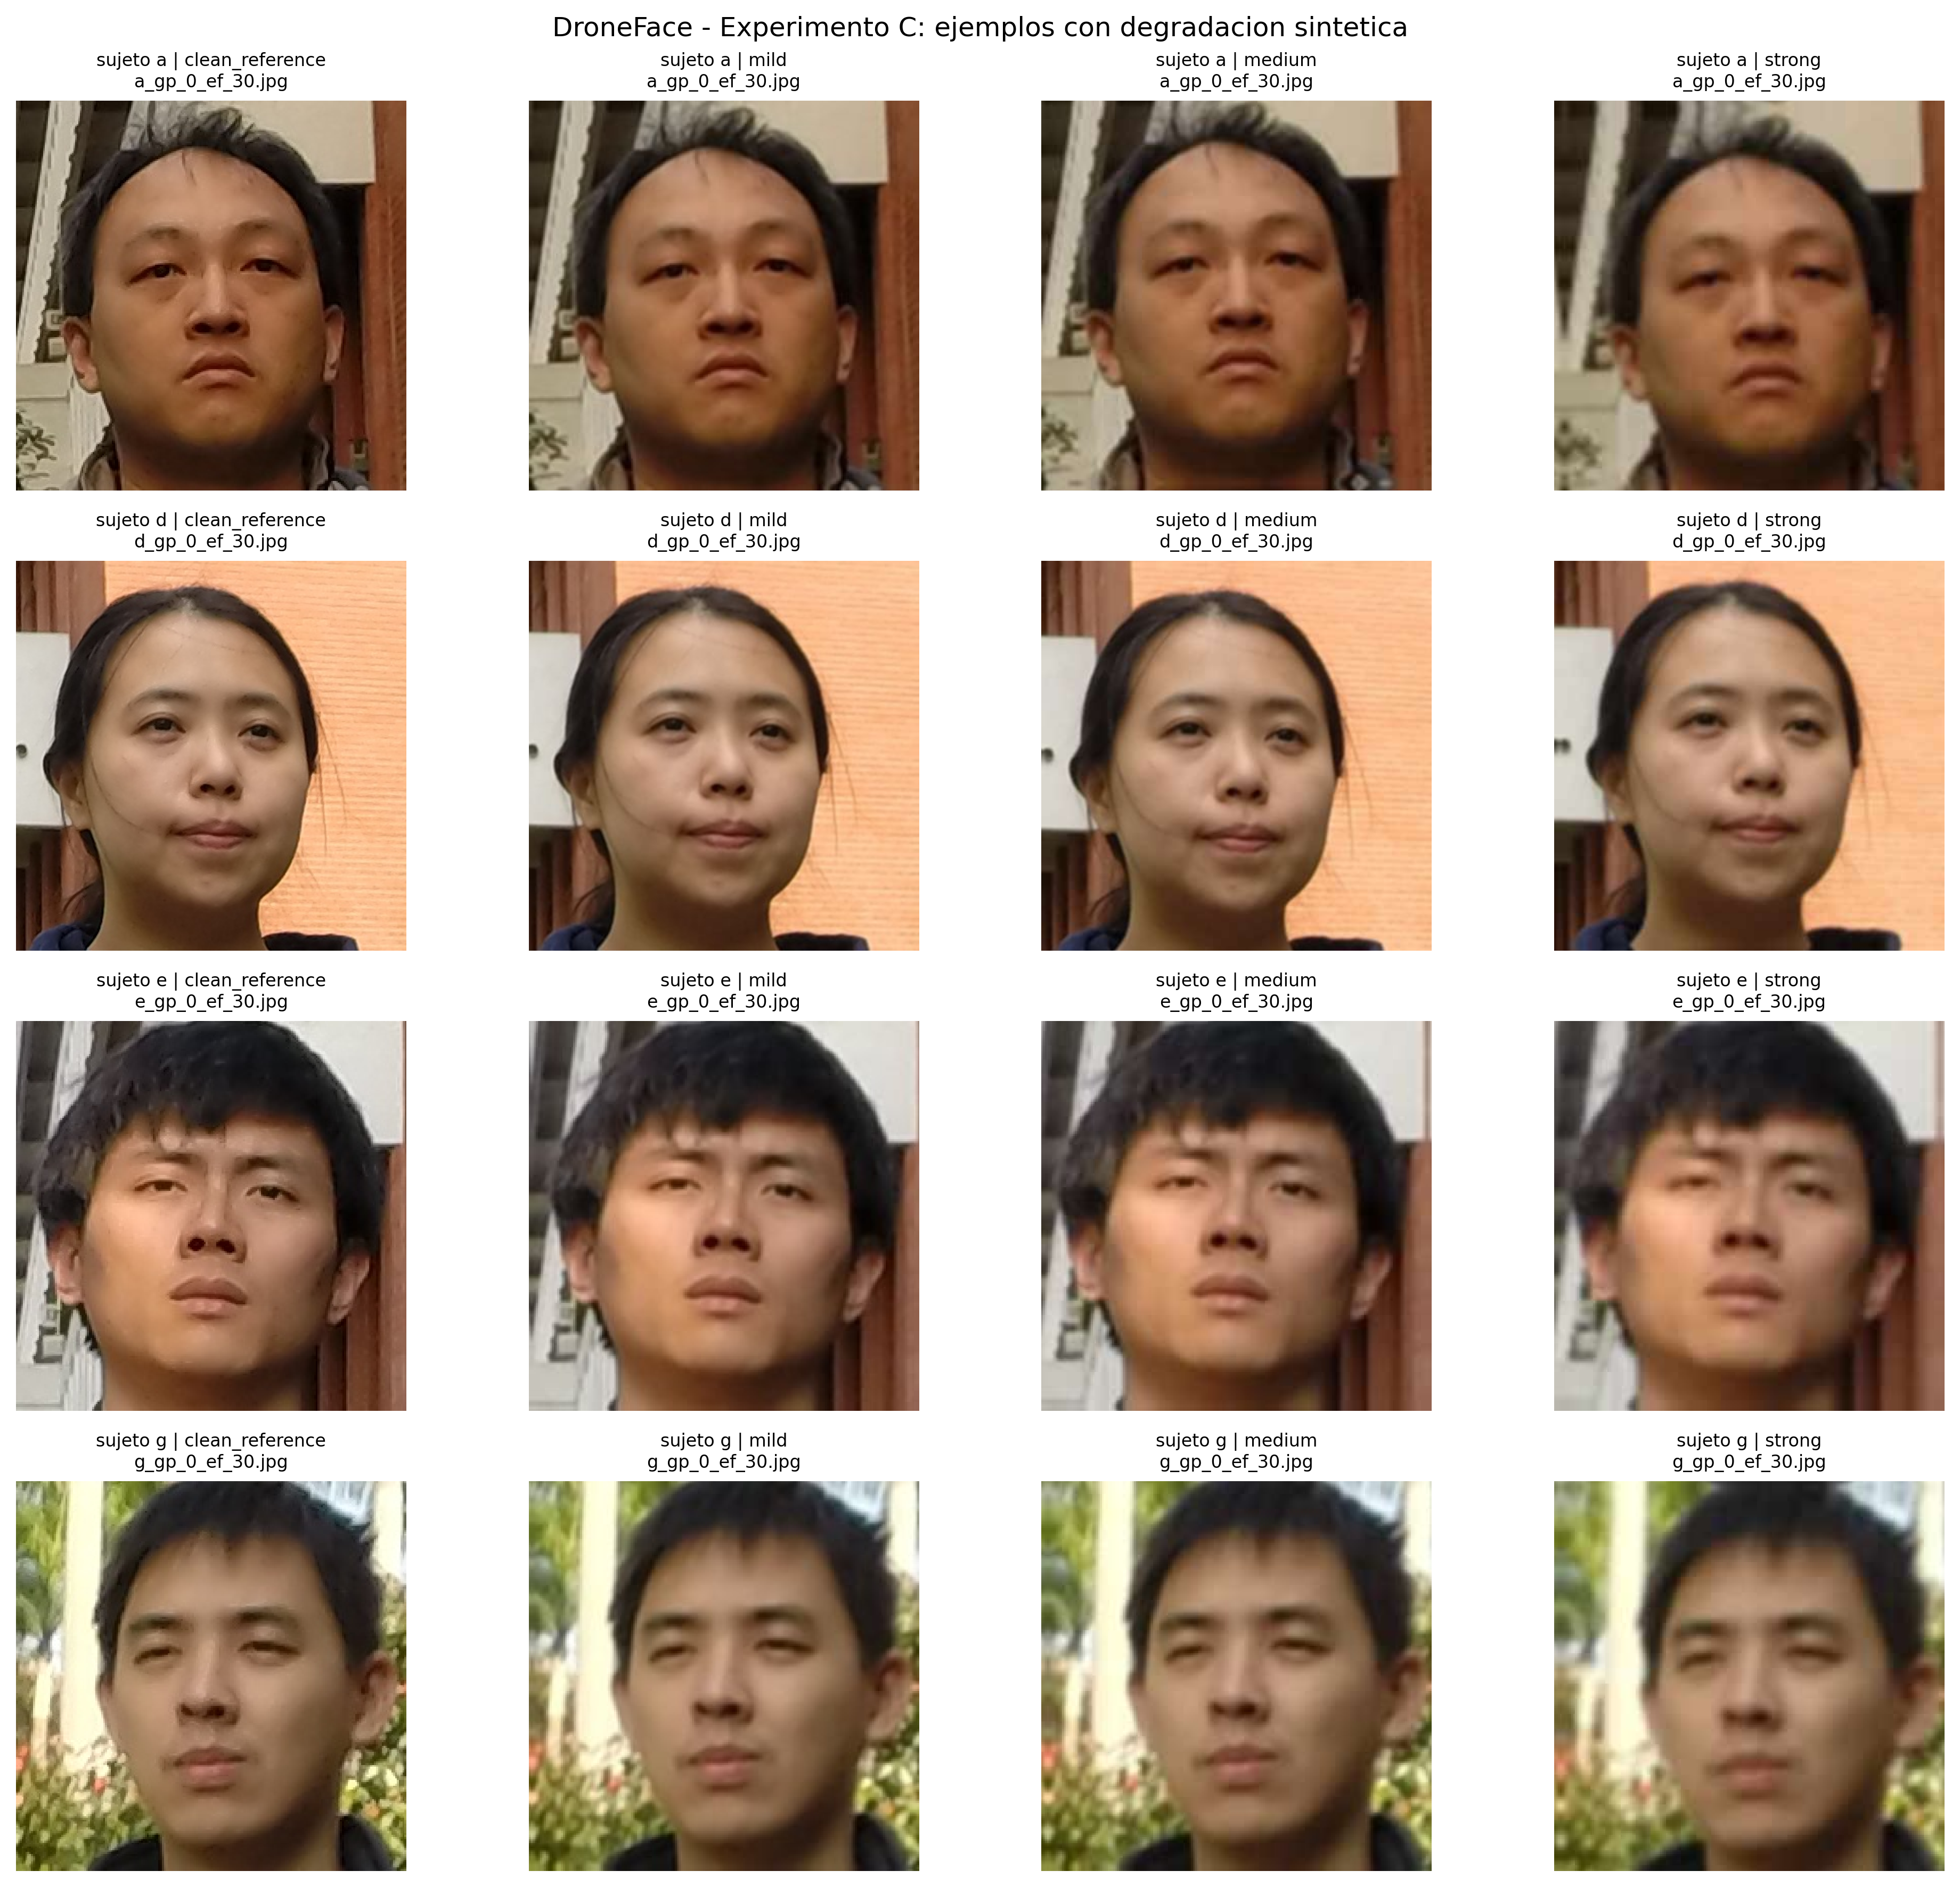
\includegraphics[width=\textwidth]{recognition/droneface_synthetic_degradation_examples.png}
\caption{Ejemplos de probes sintéticos usados en el Experimento C.}
\label{fig:exp_c_examples}
\end{figure}

\subsection{Sensibilidad del detector en rostros recortados}

También se realizó un barrido de \texttt{det\_size} en el protocolo del Experimento A. A diferencia del caso de imágenes completas, aumentar \texttt{det\_size} no mejoró el desempeño en estos rostros recortados. Como se observa en la Tabla~\ref{tab:det_size_a}, el mejor resultado se obtuvo con \texttt{det\_size=320}; por eso esa configuración quedó como baseline para A y para el Experimento C.

\begin{table}[H]
\centering
\caption{Barrido de \texttt{det\_size} para el protocolo del Experimento A.}
\label{tab:det_size_a}
\begin{tabular}{cccc}
\toprule
\texttt{det\_size} & \texttt{detection\_rate} & \texttt{accuracy\_conditional} & \texttt{accuracy\_global} \\
\midrule
320 & 99.31\% & 91.42\% & 90.78\% \\
640 & 55.99\% & 87.24\% & 48.85\% \\
1024 & 0.27\% & 0.00\% & 0.00\% \\
\bottomrule
\end{tabular}
\end{table}

La Figura~\ref{fig:det_size_a} resume el mismo barrido. Este resultado debe interpretarse como una sensibilidad empírica de esta implementación y de esta copia de DroneFace, no como una propiedad universal de InsightFace. En estos recortes ya centrados y de baja resolución, aumentar la entrada del detector puede alterar la escala efectiva con que se procesa la imagen y perjudicar la detección.

\begin{figure}[H]
\centering
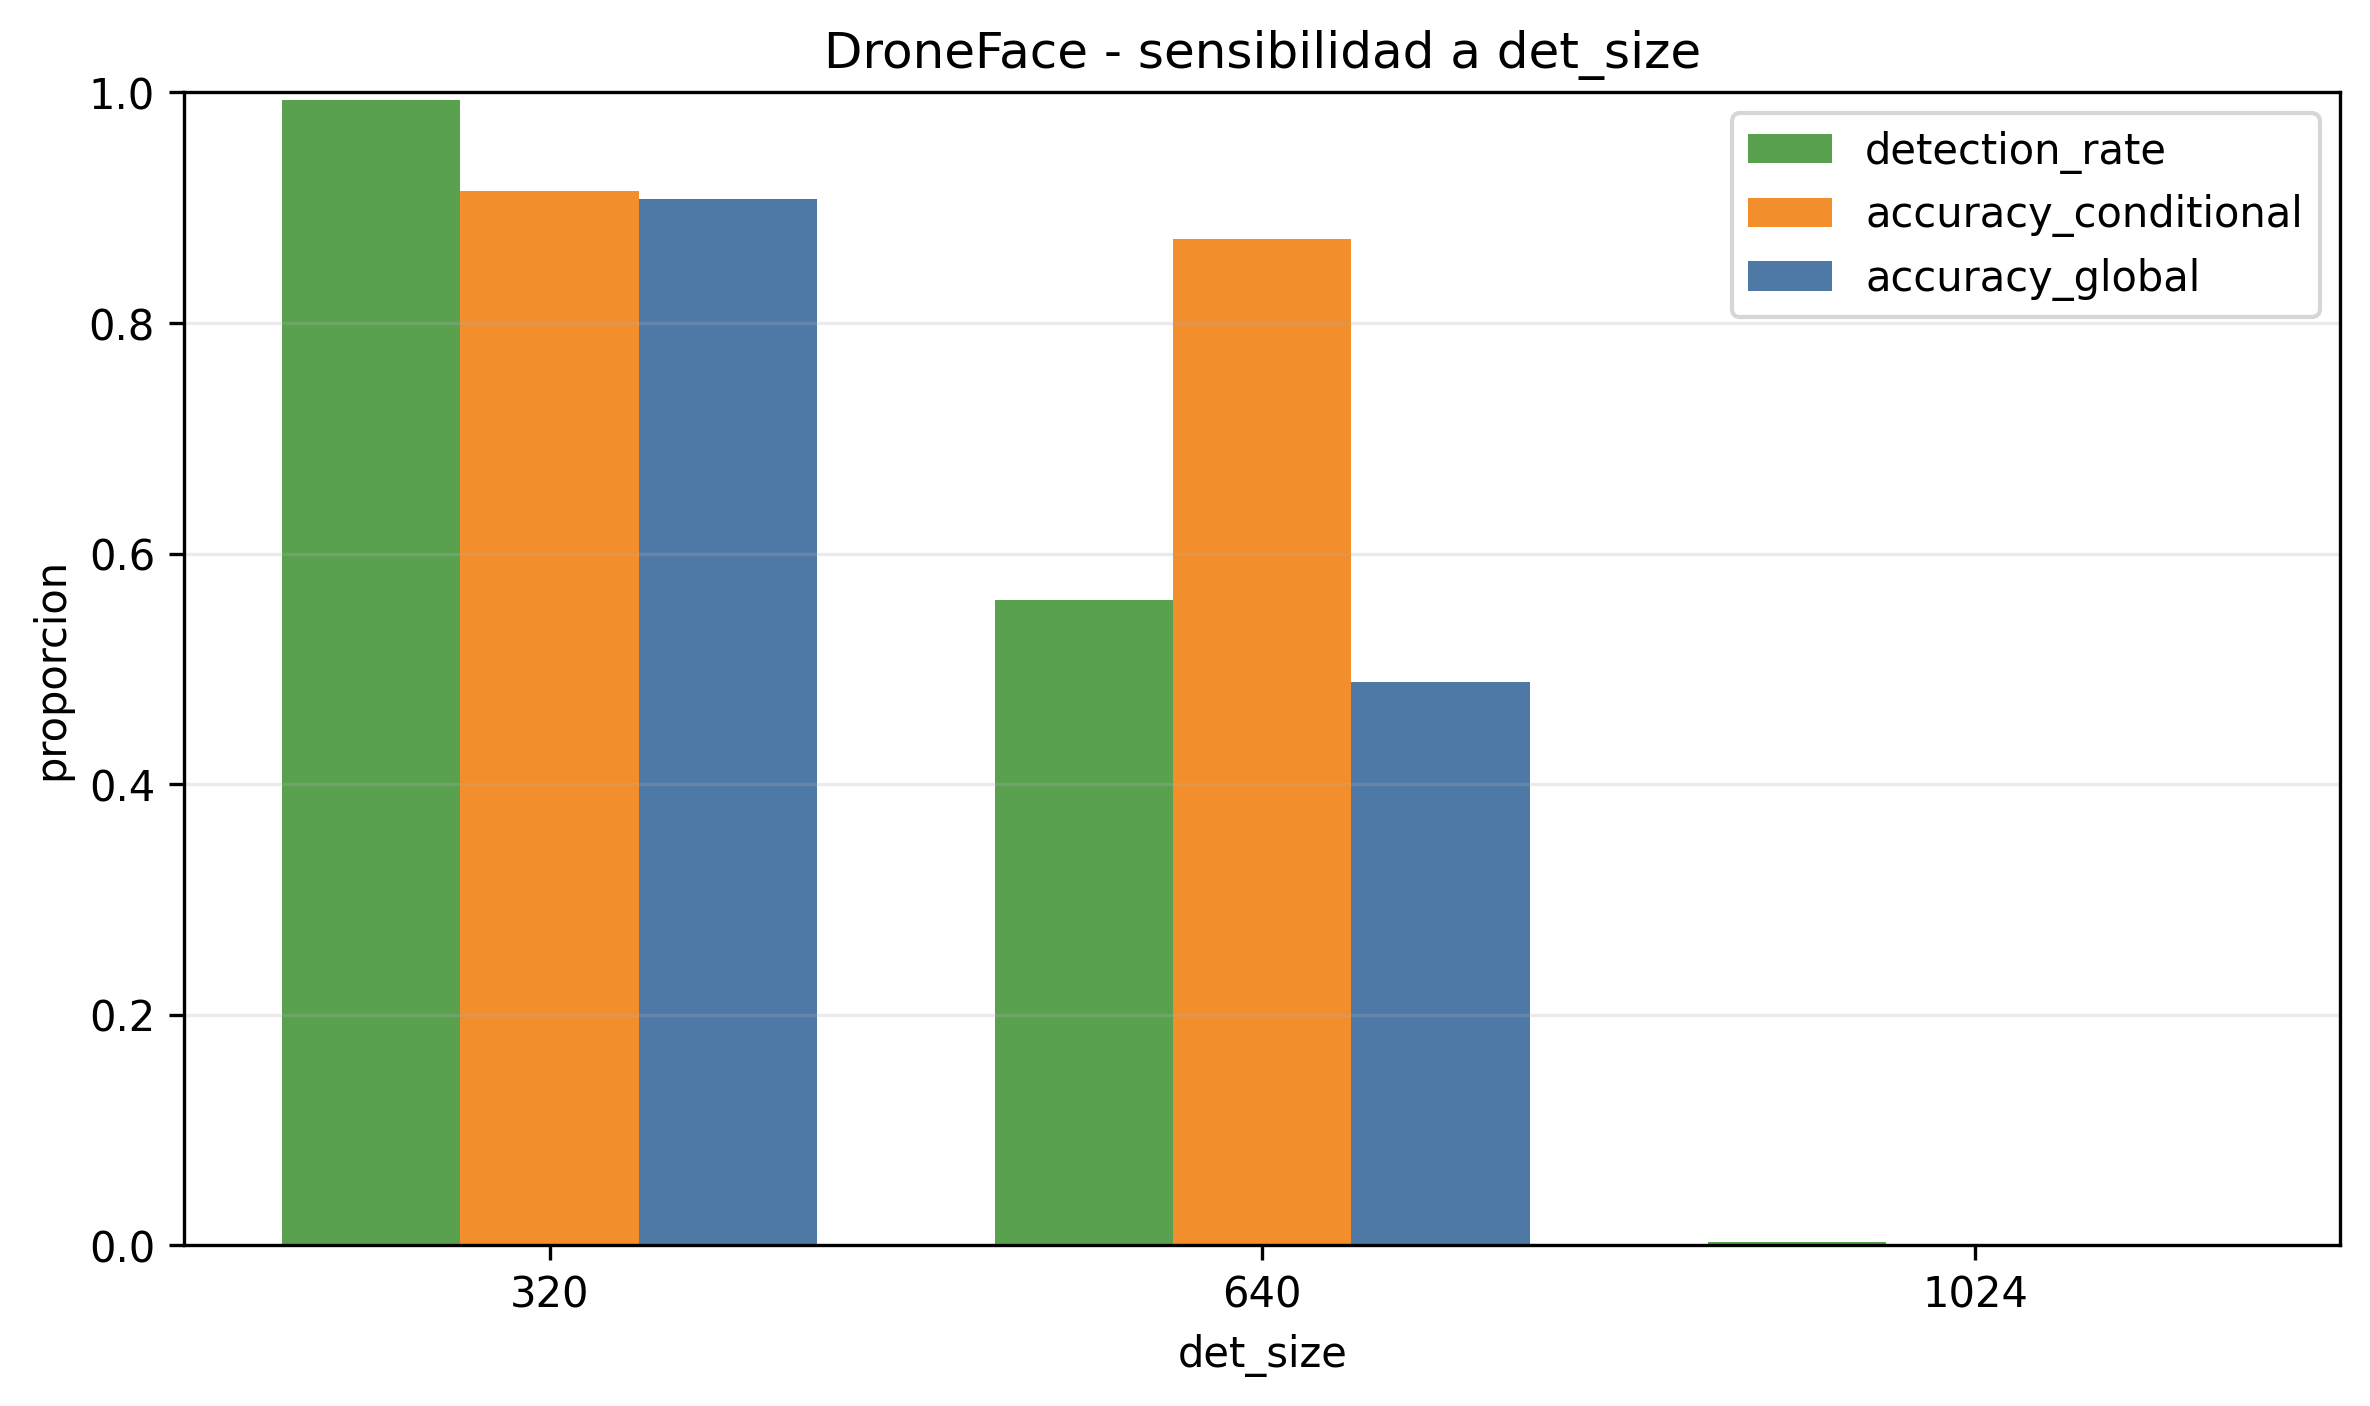
\includegraphics[width=0.95\textwidth]{metrics/droneface_det_size_detection_accuracy.png}
\caption{Sensibilidad del Experimento A frente al parámetro \texttt{det\_size}.}
\label{fig:det_size_a}
\end{figure}

\section{Discusión}
\label{sec:discusion}

El Experimento A demuestra que el reconocimiento \textit{closed-set} funciona razonablemente bien cuando el rostro ya está recortado y la identidad pertenece a la galería. Como se observa en la Tabla~\ref{tab:exp_a_global}, la \texttt{accuracy\_global} de 90.78\% indica que ArcFace/InsightFace es un baseline fuerte para este conjunto. Sin embargo, las Figuras~\ref{fig:exp_a_distancia} y~\ref{fig:heatmap_a} muestran que el desempeño cae con distancia y altura, especialmente cuando el rostro pierde resolución efectiva. La Tabla~\ref{tab:exp_a_sujeto} y la Figura~\ref{fig:confusion_a} muestran además que el error depende del sujeto: algunas identidades se reconocen de forma casi perfecta, mientras que otras se confunden con mayor frecuencia.

El Experimento B es más difícil y debe interpretarse con cuidado. En este caso el sistema debe resolver detección y reconocimiento dentro de una imagen completa. Además, la verdad terreno disponible solo indica el conjunto de identidades presentes en la imagen, no la identidad de cada rostro detectado. Por eso no se puede afirmar que una caja específica sea un verdadero positivo o un falso positivo. La Tabla~\ref{tab:exp_b} responde una pregunta más débil: cuántas identidades esperadas logró recuperar el sistema en cada imagen. La Figura~\ref{fig:full_detections} ayuda a revisar visualmente el proceso, pero no convierte la evaluación en una medición por instancia.

El Experimento C complementa esta limitación. Al degradar imágenes con identidad conocida, se mide el reconocimiento de forma controlada. La Tabla~\ref{tab:exp_c} y la Figura~\ref{fig:exp_c_rank1} muestran un descenso desde 100.00\% en la referencia limpia hasta 74.29\% con degradación fuerte. Esto sugiere que el módulo de reconocimiento es sensible a blur, compresión y pérdida de resolución, y apoya la hipótesis de que parte de la caída observada en B proviene de la calidad visual de los rostros detectados. Sin embargo, C no debe leerse como desempeño absoluto sobre todo DroneFace, sino como sensibilidad relativa al degradar casos inicialmente reconocibles.

Finalmente, las Tablas~\ref{tab:det_size_a} y~\ref{tab:det_size_b} justifican la configuración final del detector. Se usó \texttt{det\_size=320} en A y C porque fue la mejor configuración sobre recortes, mientras que B usa \texttt{det\_size=1280} porque fue la mejor configuración en imágenes completas. Por lo tanto, el informe no reporta una configuración arbitraria, sino la mejor configuración encontrada dentro del barrido realizado.

\subsection{Limitaciones}

La evaluación queda limitada por la disponibilidad local de datos y anotaciones. Primero, no se usó SCface porque no está disponible localmente, de modo que las conclusiones se restringen a DroneFace. Segundo, la galería principal contiene solo 7 sujetos porque \texttt{portraits} no incluye referencias para \texttt{b}, \texttt{c}, \texttt{f} y \texttt{h}. El protocolo maneja esto filtrando A y C, y separando en B las identidades esperadas con y sin galería.

La limitación más importante del Experimento B es que \texttt{photos\_all} no contiene anotaciones de identidad por bounding box. Por ello, no se pueden medir TP, FP, FN, precisión, recall ni F1 reales por rostro detectado. El Experimento C también tiene una limitación propia: usa probes inicialmente reconocibles, por lo que mide sensibilidad ante degradación, no desempeño absoluto sobre todos los casos posibles.

Finalmente, \texttt{trio\_cam} y \texttt{trio\_gp} quedan fuera del protocolo principal porque requerirían definir una galería alternativa multi-vista o multi-cámara. Tampoco se evalúa un escenario \textit{open-set}: no existe umbral de desconocido y toda detección se asigna a la identidad más cercana dentro de la galería.

\section{Conclusiones}
\label{sec:conclusiones}

Se implementó un baseline reproducible de reconocimiento facial sobre DroneFace usando InsightFace/ArcFace preentrenado. El protocolo separa tres niveles de dificultad: reconocimiento sobre rostros recortados, recuperación de identidades en imágenes completas y reconocimiento controlado bajo degradación sintética. Además, se verificó que el mismo paquete \texttt{buffalo\_l} contiene submodelos distintos para detección y reconocimiento, y se ajustó \texttt{det\_size} según el tipo de entrada.

El pipeline genera índices, tablas y figuras de forma reproducible, por lo que puede reejecutarse al cambiar la copia del dataset, el modelo de reconocimiento o la configuración de detección.

Los resultados principales son:

\begin{itemize}
    \item En rostros recortados, el sistema alcanza 90.78\% de \texttt{accuracy\_global}.
    \item En imágenes completas, recupera 78.80\% de las identidades esperadas con galería, pero esta métrica no equivale a accuracy por rostro.
    \item Bajo degradación sintética fuerte, el \rankone{} baja a 74.29\%, mostrando sensibilidad al ruido visual.
\end{itemize}

El principal aprendizaje metodológico es que el Experimento B no debe presentarse como evaluación de clasificación por instancia, ya que faltan anotaciones de identidad por bounding box. La forma correcta de reportarlo es como recuperación de identidades con supervisión débil. Como trabajo futuro, se recomienda etiquetar manualmente los crops o bounding boxes del Experimento B. Con esa anotación se podrían medir TP, FP, FN, precisión, recall y F1 reales por rostro detectado. También sería útil evaluar un protocolo \textit{open-set}, incorporar umbrales de desconocido y comparar ArcFace con otros modelos de reconocimiento facial.

\newpage
\bibliographystyle{ieeetr}
\bibliography{referencias}

\end{document}
